%%% JCAP-style standalone paper
%%% Target: Journal of Cosmology and Astroparticle Physics
\documentclass[a4paper,11pt]{article}
\usepackage[utf8]{inputenc}
\usepackage[T1]{fontenc}
\usepackage{amsmath,amssymb,amsthm,mathtools,bm}
\usepackage{graphicx}
\usepackage[margin=2.5cm]{geometry}
\usepackage{hyperref}
\usepackage{booktabs}
\usepackage{xcolor}
\usepackage{float}
\usepackage{caption}

\hypersetup{colorlinks=true,linkcolor=blue!60!black,citecolor=green!50!black,urlcolor=blue!70!black}
\graphicspath{{figures/}}

%%% Macros
\newcommand{\Sig}{\Sigma}
\newcommand{\SigH}{\Sigma_H}
\newcommand{\Yp}{Y_p}
\newcommand{\Neff}{N_{\rm eff}}
\newcommand{\Teff}{T_{\rm eff}}
\newcommand{\FLRW}{\mathrm{FLRW}}
\newcommand{\dd}{\mathrm{d}}
\newcommand{\order}{\mathcal{O}}
\newcommand{\GF}{G_{\rm F}}
\newcommand{\sw}{\sin^2\!\theta_{\rm W}}

\title{\textbf{Self-consistent Big Bang nucleosynthesis\\[4pt]
in Bianchi Type~I cosmology.~I.~Formalism and constraints}}
\author{}
\date{}

\begin{document}
\maketitle

%%% ====================================================================
%%%  ABSTRACT
%%% ====================================================================
\begin{abstract}
\noindent
We present a self-consistent computation of primordial nucleosynthesis in Bianchi Type~I spacetime, solving the coupled Einstein--Boltzmann--nuclear system without approximating the neutrino transport or fixing the shear decay law \textit{a priori}.  The production code RABBIT (\textbf{R}osenbrock \textbf{A}daptive \textbf{BB}N with \textbf{B}ianchi-type \textbf{I}ntegration \textbf{T}oolkit) evolves the Wainwright--Hsu Hubble-normalised shear variables, exact characteristic neutrino transport with full momentum dependence, weak $n\leftrightarrow p$ rates with Coulomb and Sirlin radiative corrections, the Bennett QED equation of state, and the PRIMAT AC2024 nuclear network as a single stiff ODE system.

Three principal results emerge.  First, the self-consistent shear decay law during radiation domination is $\sigma \propto a^{-5/2}$, not the $a^{-3}$ assumed in all prior BBN anisotropy analyses.  The slower decay originates from the neutrino viscous reservoir: free-streaming neutrinos store shear energy in their quadrupole moment and release it back to the geometry on a timescale $\sim$1.5~e-folds.  Second, exact characteristic transport reveals a 27--36\% nonlinear correction to the helium-4 yield beyond the linearised PSTF hierarchy, arising from momentum-dependent spectral distortion that is invisible to $q$-independent multipole variables.  Third, using observed abundances $\Yp = 0.2449 \pm 0.0040$ and $\mathrm{D/H} = (2.547 \pm 0.029)\times 10^{-5}$, we derive $\SigH < 0.66$ at 95\% CL (profile likelihood, CL2 corrections).  The FLRW baseline is recovered with PRIMAT parity $|\Delta\Yp| = 6.7\times 10^{-5}$.

\vspace{6pt}
\noindent\textbf{Keywords:} Big Bang nucleosynthesis, Bianchi cosmologies, neutrino transport, primordial anisotropy
\end{abstract}

\newpage
\tableofcontents
\newpage

%%% ====================================================================
%%%  1. INTRODUCTION
%%% ====================================================================
\section{Introduction}\label{sec:intro}

Big Bang nucleosynthesis (BBN) is one of the three observational pillars of hot big bang cosmology.  The standard calculation assumes a Friedmann--Lema\^itre--Robertson--Walker (FLRW) spacetime and has been developed to sub-percent precision by dedicated codes such as PRIMAT~\cite{PitrouPRIMAT2021}, \textsc{PArthENoPE}~\cite{PArthENoPE2018}, and \textsc{AlterBBN}~\cite{AlterBBN2020}.  The predicted primordial helium-4 mass fraction $\Yp$ is a sensitive probe of the expansion rate at temperatures $T \sim 0.01$--10~MeV, depending on the neutron lifetime $\tau_n$, the baryon-to-photon ratio $\eta$, the effective number of neutrino species $\Neff$, and the details of weak $n\leftrightarrow p$ interconversion.

While the cosmic microwave background (CMB) constrains spatial anisotropy at one part in $10^5$ at recombination, this is a late-time bound: the universe at BBN temperatures could have been significantly more anisotropic, with the shear subsequently decaying.  The question of how much primordial anisotropy is compatible with observed light-element abundances has acquired renewed relevance in light of the hemispherical power asymmetry in the CMB~\cite{Planck2020anomalies}, the persistent Hubble tension~\cite{Riess2022}, and the anomalous quasar dipole~\cite{Secrest2022}.

The effect of anisotropy on BBN was first studied by Barrow~\cite{Barrow1976}, who noted that shear energy density enters the Friedmann equation as additional radiation, accelerating the expansion and raising $\Yp$.  The back-reaction of neutrino anisotropic stress---the Misner viscosity~\cite{Misner1968}---was incorporated by Rothmann and Matzner~\cite{RothmannMatzner1984} in a linearised treatment.  More recently, Park et~al.~\cite{Park2025} revisited the problem with modern nuclear rates, but retained the standard assumption $\sigma \propto a^{-3}$ for the shear decay law.

All these analyses share a common limitation: the shear evolution is not solved self-consistently with the neutrino transport.  Instead, a decay law is imposed and the neutrino anisotropic stress is either neglected or treated perturbatively.  This paper removes that limitation.  We solve the full coupled system---geometry, neutrino transport, weak rates, and nuclear network---as a single stiff initial-value problem, making no assumptions about the functional form of $\sigma(a)$.

Three results follow that were inaccessible to prior treatments:
\begin{enumerate}
\item The self-consistent decay law is $\sigma \propto a^{-5/2}$, not $a^{-3}$.  This weakens the extrapolation of BBN constraints to the present epoch by three to four orders of magnitude.
\item Exact characteristic transport captures a 27--36\% nonlinear correction to $\Yp$ beyond the linearised PSTF hierarchy, arising from $q$-dependent spectral hardening.
\item The constraint on the Hubble-normalised shear is $\SigH < 0.66$ (95\% CL) with Coulomb and Sirlin radiative corrections (CL2), substantially weaker than previously reported values that assumed $a^{-3}$ scaling.
\end{enumerate}

The Bianchi classification provides the natural framework for spatially homogeneous but anisotropic cosmologies~\cite{WainwrightEllis1997}.  Type~I, the simplest anisotropic generalisation of flat FLRW, has three independent scale factors and serves as a controlled laboratory for studying the geometry--transport--nucleosynthesis coupling chain.  Extensions to curved Bianchi types (II, VI$_0$, VII$_0$, VIII, IX) are deferred to future work.

The remainder of this paper is organised as follows.  Section~\ref{sec:geometry} presents the Bianchi Type~I geometry in the Wainwright--Hsu dynamical-systems formulation.  Section~\ref{sec:transport} derives the neutrino transport equations in both the linearised PSTF hierarchy and the exact method of characteristics.  Section~\ref{sec:eigenvalues} analyses the eigenvalue structure of the coupled shear--stress system and derives the $a^{-5/2}$ decay law.  Section~\ref{sec:numerics} describes the RABBIT code and its validation.  Section~\ref{sec:results} presents the BBN yields, nonlinear correction, and observational constraints.  Section~\ref{sec:discussion} discusses implications and compares with prior work.  Section~\ref{sec:conclusions} summarises.


%%% ====================================================================
%%%  2. BIANCHI TYPE I GEOMETRY
%%% ====================================================================
\section{Bianchi Type~I geometry}\label{sec:geometry}

In the orthonormal-frame approach of Wainwright and Hsu~\cite{WainwrightEllis1997}, the Bianchi Type~I spacetime has the diagonal metric
\begin{equation}
\dd s^2 = -\dd t^2 + a_1(t)^2\,\dd x^2 + a_2(t)^2\,\dd y^2 + a_3(t)^2\,\dd z^2\,,
\end{equation}
where the mean scale factor is $a = (a_1 a_2 a_3)^{1/3}$ and the mean Hubble rate is $H = \dot{a}/a$.  The expansion tensor $\theta_{ij} = \mathrm{diag}(\dot{a}_1/a_1,\,\dot{a}_2/a_2,\,\dot{a}_3/a_3)$ decomposes into its trace $\theta = 3H$ and the traceless shear tensor $\sigma_{ij} = \theta_{ij} - H\,\delta_{ij}$.  The two algebraically independent components of the shear are conventionally packaged as $\sigma_+ = (\sigma_{11} - \sigma_{22})/2$ and $\sigma_- = \sigma_{33}/(2\sqrt{3})$.  Introducing the Hubble-normalised shear variables
\begin{equation}
\Sig_\pm = \frac{\sigma_\pm}{H}\,,\qquad \Sig^2 \equiv \Sig_+^2 + \Sig_-^2\,,
\end{equation}
the dynamical equations take the form of an autonomous system in the e-fold time $N = \ln a$.

\textit{Derivation of the shear evolution equation.}  The Einstein field equations for Bianchi Type~I, projected onto the traceless part of the spatial $(ij)$ components, yield the shear propagation equation
\begin{equation}
\dot{\sigma}_{ij} + 3H\,\sigma_{ij} = -\pi_{ij}\,,\label{eq:shear_prop_cosmic}
\end{equation}
where $\pi_{ij}$ is the traceless anisotropic stress tensor of the matter content.  Converting to e-fold time via $\dot{X} = H\,\dd X/\dd N$ and defining $\Sig_\pm = \sigma_\pm / H$ as well as $\Pi_\pm = \pi_\pm / (3H^2)$, one obtains by the quotient rule
\begin{equation}
\frac{\dd\Sig_\pm}{\dd N} = \frac{1}{H}\frac{\dd\sigma_\pm}{\dd N} - \frac{\sigma_\pm}{H^2}\frac{\dd H}{\dd N}
= \frac{\dot{\sigma}_\pm}{H^2} - \Sig_\pm\,\frac{\dot{H}}{H^2}\,.
\end{equation}
Substituting \eqref{eq:shear_prop_cosmic} for $\dot\sigma_\pm$ and using the Raychaudhuri equation $\dot{H}/H^2 = -(1+q)$ where $q$ is the deceleration parameter,
\begin{equation}
\frac{\dd\Sig_\pm}{\dd N} = \frac{-3H\,\sigma_\pm - \pi_\pm}{H^2} + (1+q)\,\Sig_\pm
= -3\,\Sig_\pm - \frac{\pi_\pm}{H^2} + (1+q)\,\Sig_\pm\,.
\end{equation}
During radiation domination with anisotropic stress, $q = 1 + \Sig^2$ (this follows from the Raychaudhuri equation with $\rho + 3p = 2\rho$ for radiation and the shear contribution $2\sigma^2$).  Collecting terms and identifying $\Pi_\pm = \pi_\pm/(3H^2)$:
\begin{equation}
\frac{\dd\Sig_+}{\dd N} = -(2-q)\,\Sig_+ + \Pi_+\,,\qquad
\frac{\dd\Sig_-}{\dd N} = -(2-q)\,\Sig_- + \Pi_-\,,\label{eq:dSig}
\end{equation}
where the coefficient $-(2-q) = -(1-\Sig^2)$ reduces to $-1$ at linear order.  The source $\Pi_\pm$ is the Hubble-normalised neutrino anisotropic stress, which provides the viscous back-reaction of free-streaming neutrinos on the geometry.  In the absence of anisotropic stress ($\Pi_\pm = 0$), $\Sig$ decays as $e^{-N}$ at linear order, corresponding to the free-decay law $\sigma \propto a^{-3}$ ($\rho_\sigma \propto a^{-6}$).

\textit{Derivation of the Friedmann constraint.}  The $(00)$ Einstein equation gives the Friedmann equation
\begin{equation}
3H^2 = \rho + \frac{1}{2}\sigma^2\,,
\end{equation}
where $\sigma^2 \equiv \sigma_{ij}\sigma^{ij} = 6H^2\Sig^2$.  Dividing by $3H^2$ and defining $\Omega \equiv \rho/(3H^2)$:
\begin{equation}
1 = \Omega + \Sig^2\qquad\Longrightarrow\qquad \Omega = 1 - \Sig^2\,,\label{eq:friedmann}
\end{equation}
with $\Omega = \rho/(3H^2)$ the total density parameter.  This is enforced algebraically at each timestep.

\textit{Derivation of the Hubble enhancement.}  The isotropic Hubble rate is defined as $H_\FLRW \equiv \sqrt{\rho/(3M_{\rm Pl}^2)}$, i.e., the Hubble rate that the same energy density $\rho$ would produce in an FLRW universe.  From the Friedmann equation $3H^2 = \rho + 3H^2\Sig^2$, solving for $H$:
\begin{equation}
3H^2(1 - \Sig^2) = \rho \qquad\Longrightarrow\qquad H^2 = \frac{\rho}{3(1 - \Sig^2)} = \frac{H_\FLRW^2}{1 - \Sig^2}\,,
\end{equation}
so that
\begin{equation}
H = \frac{H_\FLRW}{\sqrt{1 - \Sig^2}}\,.\label{eq:hubble}
\end{equation}
For small anisotropy, $\delta H/H \approx \Sig^2/2$.  This Hubble enhancement constitutes the first channel of the anisotropy--BBN coupling: faster expansion shifts weak freeze-out to earlier times, trapping more neutrons and raising $\Yp$.

The shear energy density scales as $\rho_\sigma \propto a^{-6}$ in the absence of viscosity (free decay), compared to $\rho_{\rm rad} \propto a^{-4}$.  With self-consistent neutrino viscosity, the effective scaling becomes $\rho_\sigma \propto a^{-5}$, as we derive in section~\ref{sec:eigenvalues}.  The difference---$T^5$ for shear versus $T^4$ for radiation---breaks the leading-order degeneracy $\Sig^2 \leftrightarrow \Delta\Neff$.


%%% ====================================================================
%%%  3. NEUTRINO TRANSPORT
%%% ====================================================================
\section{Neutrino transport}\label{sec:transport}

\subsection{Boltzmann equation in Bianchi Type~I}\label{sec:boltzmann_deriv}

The distribution function of massless neutrinos $f(x^a, p^a)$ obeys the Liouville equation $p^a\nabla_a f = 0$ on the mass shell $g_{ab}p^a p^b = 0$.  In the spatially homogeneous Bianchi Type~I background, $f$ depends only on the magnitude $p$ and direction of the momentum and on time.  We parametrise the momentum by the comoving variable $q = pa/T_0$ (where $T_0$ is a reference temperature) and the direction cosine $\mu = \hat{p}\cdot\hat{e}_3$ with respect to the anisotropy axis.  In these variables, the geodesic equation gives
\begin{equation}
\frac{\dd\ln q}{\dd N} = -2\,\Sig_+\,P_2(\mu)\,,\qquad
\frac{\dd\mu}{\dd N} = 3\,\Sig_+\,\mu\,(1-\mu^2)\,,\label{eq:geodesic_sources}
\end{equation}
where the first equation encodes the direction-dependent gravitational redshift (neutrinos travelling along the faster-expanding axis lose more energy) and the second encodes the focusing of rays toward the slower-expanding directions.  Substituting into the phase-space Liouville equation $\partial f/\partial N + (\dd\ln q/\dd N)\,q\,\partial f/\partial q + (\dd\mu/\dd N)\,\partial f/\partial\mu = 0$ yields
\begin{equation}
\frac{\partial f}{\partial N} + \frac{\dd\ln q}{\dd N}\,q\,\frac{\partial f}{\partial q} + \frac{\dd\mu}{\dd N}\,\frac{\partial f}{\partial\mu} = 0\,.\label{eq:boltzmann}
\end{equation}
This is a first-order linear PDE in $(N, q, \mu)$, amenable to both multipole expansion and characteristic solution.

\subsection{Linearised PSTF hierarchy}\label{sec:pstf}

The Projected Symmetric Trace-Free (PSTF) formalism expands the distribution perturbation in Legendre multipoles,
\begin{equation}
f(q,\mu,N) = f_0(q)\Bigl[1 + \sum_{\ell\,{\rm even}} \Psi_\ell(q,N)\,P_\ell(\mu)\Bigr]\,,
\end{equation}
where $f_0(q) = [e^q+1]^{-1}$ is the equilibrium Fermi--Dirac distribution and odd multipoles vanish by the $\mu \to -\mu$ symmetry of axisymmetric Type~I.

\textit{Derivation of the hierarchy.}  Substituting the multipole expansion into~\eqref{eq:boltzmann} and projecting onto $P_\ell(\mu)$ using the orthogonality relation $\int_{-1}^{1} P_\ell P_{\ell'}\,\dd\mu = 2\delta_{\ell\ell'}/(2\ell+1)$, the $q\,\partial f/\partial q$ source term produces the coupling.  At linear order in $\Sig$, the $q$-derivative acts on $f_0(q)$ and generates a factor $-q\,f_0'(q)/f_0(q)$ that is common to all multipoles.  For the $q$-independent PSTF variable $\Psi_\ell$, this factor cancels after energy weighting, leaving:
\begin{align}
\frac{\dd\Psi_0}{\dd N} &= 0\,,\label{eq:psi0}\\[4pt]
\frac{\dd\Psi_2}{\dd N} &= -\frac{8}{15}\,\Sig_+ - D\,\Psi_2\,.\label{eq:psi2}
\end{align}
The monopole equation $\dot\Psi_0 = 0$ follows because the $P_0$ projection of $P_2(\mu)$ vanishes.  The quadrupole source coefficient $-8/15$ arises from the overlap integral $\int P_2 P_2\,\dd\mu = 2/5$ combined with the redshift coupling $-2\Sig_+$, giving $-2\Sig_+ \times (2/5) \times (2\ell+1)/2 = -8\Sig_+/15$.  The damping $D\,\Psi_2$ with $D = 4$ comes from the angular redistribution term $(\dd\mu/\dd N)\,\partial f/\partial\mu$: the $P_2 \to P_2$ self-coupling gives $D = 6\Sig_+ \times 2/5 \times 5 = 4\Sig_+$, normalised to $D = 4$ at leading order.

A remarkable property of Bianchi Type~I is that the collisionless hierarchy \emph{closes exactly} at $\ell_{\max} = 2$: the geometric source term $P_2(\mu)$ couples $\ell$ to $\ell \pm 2$ only, and the $\ell = 2 \to \ell = 4$ coupling coefficient vanishes identically for flat spatial sections (zero spatial curvature $\Rightarrow$ zero $\kappa_\ell^m$ connection coefficients).  Thus $\Psi_4 = \Psi_6 = \cdots = 0$ is a self-consistent solution, and the hierarchy truncates without approximation.

\textit{Derivation of the anisotropic stress.}  The neutrino anisotropic stress $\pi_{ij}$ is the traceless second moment of the distribution function.  For a single species, the $P_2$-weighted energy moment gives
\begin{equation}
\tilde\pi = \frac{\int_0^\infty \dd q\,q^3\,\int_{-1}^{1}\dd\mu\,P_2(\mu)\,f(q,\mu)}{\int_0^\infty \dd q\,q^3\,\int_{-1}^{1}\dd\mu\,f(q,\mu)}
= \frac{\int_0^\infty \dd q\,q^3 f_0(q)\,\Psi_2(q) \cdot (2/5)}{\int_0^\infty \dd q\,q^3 f_0(q) \cdot 2}\,.
\end{equation}
The Hubble-normalised stress, summed over three neutrino species and accounting for the normalisation conventions of~\cite{WainwrightEllis1997}, is
\begin{equation}
\Pi_+ = 6\,f_\nu\,\bar{\tilde\pi}\,,\qquad \bar{\tilde\pi} = \frac{\int_0^\infty \dd q\,q^3 f_0(q)\,\Psi_2(q)}{\int_0^\infty \dd q\,q^3 f_0(q)}\,,\label{eq:stress_pstf}
\end{equation}
where $f_\nu = \rho_\nu/\rho_{\rm rad} = 0.4052$ for three Standard Model neutrino species.  The factor $6$ combines $4\pi/3$ from the angular integration normalisation with $\rho_\nu/(4\pi)$, and the energy weighting $q^3$ arises from $\rho \propto \int q^3 f\,\dd q$ for massless particles.

\subsection{Exact characteristic transport}\label{sec:characteristic}

\textit{Derivation of the characteristic solution.}  The Boltzmann equation~\eqref{eq:boltzmann} with source terms~\eqref{eq:geodesic_sources} is a first-order linear PDE whose characteristics are the geodesic trajectories in $(q, \mu)$ space.  Along a characteristic labelled by the initial direction $\mu_j(0)$, the comoving momentum evolves as $q(N) = q(0)\,\exp(-2\mathcal{I}_j)$ where
\begin{equation}
\frac{\dd\mathcal{I}_j}{\dd N} = \Sig_+\,P_2(\mu_j)\,.\label{eq:dI}
\end{equation}
Since $f$ is constant along characteristics (Liouville's theorem), we have $f(q(N), \mu_j(N), N) = f(q(0), \mu_j(0), 0)$.  Assuming isotropic Fermi--Dirac initial conditions $f(q, \mu, 0) = f_{\rm FD}(q) = [e^q + 1]^{-1}$, the solution along ray $j$ is
\begin{equation}
f_j(q,N) = f_{\rm FD}\!\left(\frac{q}{\Theta_j(N)}\right)\,,\qquad \Theta_j(N) = \exp\!\bigl(-2\mathcal{I}_j(N)\bigr)\,,\label{eq:char_sol}
\end{equation}
which is simply a Fermi--Dirac distribution with a direction-dependent effective temperature $\Theta_j$.  Neutrinos travelling along directions where $P_2(\mu_j) > 0$ (polar) are blueshifted ($\Theta_j > 1$, hotter), while those with $P_2(\mu_j) < 0$ (equatorial) are redshifted ($\Theta_j < 1$, cooler).

Each ray $j$ is labelled by its initial direction cosine $\mu_j(0) \in [-1,1]$, chosen as the nodes of a Gauss--Legendre quadrature with $N_\mu$ points.  The direction cosine $\mu_j(N)$ is reconstructed analytically from the anisotropic expansion history rather than integrated as a differential equation, avoiding error accumulation.

The state per ray is the pair $(\mathcal{I}_j, J_j)$, where $J_j$ is a Jacobian factor encoding the angular redistribution of rays due to anisotropic expansion.  The total state vector for $N_\mu = 12$ rays has $2N_\mu + 1 = 25$ transport degrees of freedom, compared to $6\times 2\times N_q = 960$ for the PSTF hierarchy at $N_q = 80$ momentum nodes.

\textit{Derivation of observables.}  Physical observables are computed by angular quadrature without multipole truncation.  The anisotropic stress requires computing the $P_2$-weighted energy moment of the full distribution $f = \sum_j w_j J_j f_j$.  Using $\rho_j \propto \Theta_j^4$ for each ray's energy density (since $\int q^3 f_{\rm FD}(q/\Theta)\,\dd q = \Theta^4 \int u^3 f_{\rm FD}(u)\,\dd u$), and noting $\Theta_j^4 = e^{-8\mathcal{I}_j}$:
\begin{align}
\Pi_+ &= f_\nu \sum_j w_j\,J_j\,P_2(\mu_j)\,e^{-8\mathcal{I}_j}\,,\label{eq:Pi_char}\\
\tilde{f}_0(q) &= \frac{1}{2}\sum_j w_j\,J_j\,f_{\rm FD}\!\left(\frac{q}{\Theta_j}\right)\,.\label{eq:f0_char}
\end{align}
The monopole~\eqref{eq:f0_char} is a mixture of Fermi--Dirac distributions at different effective temperatures $\Theta_j$.  This mixture is manifestly $q$-dependent: it is not a Fermi--Dirac at any single temperature.  The resulting spectral distortion modifies weak-rate integrands and constitutes the second channel of the anisotropy--BBN coupling.

The convergence in $N_\mu$ is geometric: successive differences at $N_\mu = 8, 12, 16, 24$ are $1.5\times 10^{-5}$, $1.4\times 10^{-7}$, $1.0\times 10^{-9}$.  The FLRW limit is recovered to $|\Delta\Yp| < 7\times 10^{-10}$.


%%% ====================================================================
%%%  4. EIGENVALUE ANALYSIS
%%% ====================================================================
\section{Eigenvalue analysis}\label{sec:eigenvalues}

The linearised dynamics of the coupled shear--stress system can be analysed through two complementary $2\times 2$ systems, differing in their treatment of the quadrupole damping.

\subsection{Reduced system: real eigenvalues}\label{sec:eigen_reduced}

Writing the PSTF evolution~\eqref{eq:psi2} with $D = 4$ and combining with the shear equation~\eqref{eq:dSig}, the linearised system in the variables $(\Sig, \tilde\pi)$ is
\begin{equation}
\frac{\dd}{\dd N}\begin{pmatrix} \Sig \\ \tilde\pi \end{pmatrix}
= \underbrace{\begin{pmatrix} -1 & C_{\rm fb}\,f_\nu \\ C_{\rm src} & -D \end{pmatrix}}_{\mathbf{M}}
\begin{pmatrix} \Sig \\ \tilde\pi \end{pmatrix}\,,\label{eq:matrix_reduced}
\end{equation}
where $C_{\rm fb} = 24/5 = 4.8$, $C_{\rm src} = 8/15$, and $D = 4$.

\textit{Origin of the coefficients.}  The matrix element $M_{11} = -(2-q) \to -1$ at linear order (from~\eqref{eq:dSig} with $q \to 1$).  The feedback coefficient $M_{12} = C_{\rm fb}\,f_\nu = (24/5)\,f_\nu$ converts the normalised stress $\tilde\pi$ to the geometric source $\Pi_+ = 6 f_\nu \tilde\pi$, giving $M_{12} = 6f_\nu \times (4/5) = 24f_\nu/5$ after accounting for the $\ell = 2$ projection factor.  The source coefficient $M_{21} = C_{\rm src} = 8/15$ is the $-8/15$ from~\eqref{eq:psi2} with sign absorbed into the matrix convention.  The damping $M_{22} = -D = -4$ is the quadrupole self-coupling from the angular redistribution term.

The trace $\mathrm{tr}(\mathbf{M}) = -1 + (-4) = -5$ is universal (independent of $f_\nu$): it equals the sum of the geometric damping rate and the transport damping rate, both of which are fixed by the radiation-era kinematics.  For three Standard Model neutrino species ($f_\nu = 0.4052$), the eigenvalues are
\begin{equation}
\lambda_{\rm slow} = -0.687\,,\qquad \lambda_{\rm fast} = -4.313\,.\label{eq:lambdas}
\end{equation}
Both eigenvalues are real because the discriminant $\Delta = 25 - 4\,\det(\mathbf{M}) = 13.15 > 0$ (see appendix~\ref{app:eigenvalues} for the explicit calculation).  Approximately 91\% of the initial shear projects onto the slow mode; after $\sim$2~e-folds, only the slow mode survives.

\subsection{Transport system: oscillatory decay}\label{sec:eigen_transport}

Returning to the original $(\Sig, \Psi_2)$ variables without the $D = 4$ Markovian closure, the $2\times 2$ system becomes
\begin{equation}
\frac{\dd}{\dd N}\begin{pmatrix} \Sig \\ \Psi_2 \end{pmatrix}
= \underbrace{\begin{pmatrix} -1 & 6\,f_\nu \\ -8/15 & 0 \end{pmatrix}}_{\mathbf{M}_{\rm tr}}
\begin{pmatrix} \Sig \\ \Psi_2 \end{pmatrix}\,.\label{eq:matrix_transport}
\end{equation}
\textit{Derivation.}  From the shear equation~\eqref{eq:dSig} at linear order, $\dd\Sig/\dd N = -\Sig + \Pi_+ = -\Sig + 6f_\nu\,\Psi_2$, giving $M_{11} = -1$ and $M_{12} = 6f_\nu$.  From the PSTF quadrupole equation~\eqref{eq:psi2} \emph{without} the Markovian closure (i.e., dropping the $-D\,\Psi_2$ damping term, which is the self-coupling from the angular redistribution that is already implicitly included in the Liouville dynamics), $\dd\Psi_2/\dd N = -\frac{8}{15}\,\Sig_+$, giving $M_{21} = -8/15$ and $M_{22} = 0$.  The key difference from the reduced system~\eqref{eq:matrix_reduced} is that the Markovian damping $D = 4$ is \emph{not} imposed as a separate term; instead, the undamped hierarchy captures the exact PSTF dynamics at $\ell_{\max} = 2$ for Type~I.
The trace is $\mathrm{tr}(\mathbf{M}_{\rm tr}) = -1$ and the determinant is $\det = 16f_\nu/5$.  For $f_\nu > 5/64 \approx 0.078$ (always satisfied for $N_\nu \geq 1$), the discriminant is negative and the eigenvalues are complex:
\begin{equation}
\lambda = -\frac{1}{2} \pm i\omega\,,\qquad \omega = \frac{1}{2}\sqrt{\frac{64\,f_\nu}{5} - 1} \approx 1.023\;\text{rad/e-fold}\,.\label{eq:complex_lambda}
\end{equation}
\textit{Derivation.}  The eigenvalues of $\mathbf{M}_{\rm tr}$ satisfy $\lambda^2 - \mathrm{tr}\,\lambda + \det = 0$, i.e., $\lambda^2 + \lambda + 16f_\nu/5 = 0$.  By the quadratic formula, $\lambda = (-1 \pm \sqrt{1 - 64f_\nu/5})/2$.  Since $64f_\nu/5 = 64\times 0.4052/5 = 5.187 > 1$, the discriminant is $1 - 5.187 = -4.187 < 0$, giving complex eigenvalues with $\mathrm{Re}(\lambda) = -\mathrm{tr}/2 = -1/2$.  The real part is exact and $f_\nu$-independent: it depends only on $\mathrm{tr}(\mathbf{M}_{\rm tr}) = -1$, which equals $-(2-q)$ at linear order.

\textit{Connection to the decay law.}  The general solution of the linearised system is $\Sig(N) = e^{-N/2}[C_1\cos(\omega N) + C_2\sin(\omega N)]$.  Since $\Sig = \sigma/H$ and, in the radiation era, $H \propto a^{-2}$, the physical shear is $\sigma = H\,\Sig \propto a^{-2} \cdot e^{-N/2} = a^{-2} \cdot a^{-1/2} = a^{-5/2}$.  This yields the self-consistent decay law:
\begin{equation}
\boxed{|\Sig(N)| \sim e^{-N/2}\,,\qquad \sigma \propto a^{-5/2}\,,}\label{eq:decay_law}
\end{equation}
with damped oscillations at frequency $\omega \approx 1.023$~rad/e-fold.  The oscillation is a physical effect: shear drives neutrino anisotropic stress, which in turn damps the shear with a phase lag, creating an oscillatory energy exchange between the geometry and the neutrino quadrupole.  Equivalently, the shear energy density scales as $\rho_\sigma = 3H^2\Sig^2 \propto a^{-4}\cdot e^{-N} = a^{-5}$---intermediate between free decay ($a^{-6}$) and radiation ($a^{-4}$).

The two systems~\eqref{eq:matrix_reduced} and~\eqref{eq:matrix_transport} describe the same physics at different levels of approximation.  The transport system~\eqref{eq:matrix_transport} uses bare PSTF variables and captures the physical oscillatory decay.  The reduced system~\eqref{eq:matrix_reduced} incorporates a Markovian closure ($D = 4$) that converts the oscillation into overdamped decay, yielding two real eigenvalues.  Both are useful: the transport eigenvalues give the correct oscillation envelope ($a^{-5/2}$), while the reduced eigenvalues characterise the effective dissipation after transients.

\subsection{Comparison with prior work}

All published BBN anisotropy constraints~\cite{Barrow1976,RothmannMatzner1984,Park2025} assume $\sigma \propto a^{-3}$, i.e., the eigenvalue $\lambda = -1$ corresponding to free decay without neutrino back-reaction.  The self-consistent $a^{-5/2}$ is slower: the ratio $a^{-5/2}/a^{-3} = a^{1/2}$ grows with the scale factor.  Extrapolating a BBN-epoch constraint from $T \sim 1$~MeV to today ($T \sim 2.7$~K), the present-day bound weakens by a factor $(T_{\rm BBN}/T_0)^{1/2} \approx (10^9)^{1/2} \sim 3\times 10^4$.

The physical origin of the slower decay is the neutrino viscous reservoir.  Free-streaming neutrinos develop a quadrupole anisotropic stress in response to geometric shear.  This stress stores energy that would otherwise dissipate, releasing it back to the geometry on a timescale $|\lambda_{\rm slow}|^{-1} \approx 1.46$~e-folds.  The reservoir makes the total shear energy (geometric plus neutrino quadrupole) decay more slowly than either component alone.


%%% ====================================================================
%%%  5. WEAK RATES AND NUCLEAR NETWORK
%%% ====================================================================
\section{Weak rates and nuclear network}\label{sec:weak_rates}

The weak $n\leftrightarrow p$ interconversion rates are computed from live neutrino monopole distributions extracted from the characteristic transport, not from tabulated equilibrium rates.  Six channels contribute: three for $n\to p$ and three for $p\to n$.  The rate integrands are evaluated on a Gauss--Laguerre momentum grid with $N_q = 6$ nodes, using the $q$-dependent monopole~\eqref{eq:f0_char} that encodes the spectral distortion.

We implement a three-level correction hierarchy:
\begin{itemize}
\item \textbf{CL0 (Born)}: tree-level $V$--$A$ matrix elements with $G_{\rm F}^2(1+3g_A^2)$ normalisation.
\item \textbf{CL1 (+Coulomb)}: Fermi function $F(Z,E_e)$ for the final-state $e^\pm$ Coulomb interaction with the proton, implemented per channel with the correct sign of $Z$.
\item \textbf{CL2 (+Sirlin radiative)}: $\order(\alpha/\pi)$ outer radiative correction via the Sirlin $g$-function, adding $\sim$1.5\% to the total rate.
\end{itemize}
These corrections compose multiplicatively.  The Born rate is normalised to reproduce the measured neutron lifetime $\tau_n = 878.4$~s.

The nuclear network uses the PRIMAT AC2024 reaction rates~\cite{PitrouPRIMAT2021} with nine species (n, p, D, T, $^3$He, $^4$He, $^6$Li, $^7$Li, $^7$Be) and 31 reactions, reduced to the 8-species/12-reaction standard backbone for production runs.  The photon--electron thermodynamics employs the Bennett exact QED equation of state~\cite{Bennett2020} including $\order(e^2)$ and $\order(e^3)$ corrections, with the sign $\delta\rho < 0$ verified against the literature.


%%% ====================================================================
%%%  6. NUMERICAL IMPLEMENTATION
%%% ====================================================================
\section{Numerical implementation}\label{sec:numerics}

\subsection{The coupled ODE system}\label{sec:coupled}

The full state vector comprises geometry ($\Sig_+$, $\Sig_-$), neutrino transport ($2N_\mu + 1$ characteristic variables), photon temperature ($T_\gamma$), and nuclear abundances ($X_n$, $X_p$, $\ldots$), giving 37 degrees of freedom for $N_\mu = 12$.  Evolution proceeds in two phases:
\begin{enumerate}
\item \textbf{Phase~1} ($T \gtrsim 0.07$~MeV): geometry + transport + $n\leftrightarrow p$ weak rates only.
\item \textbf{Phase~2} ($T \lesssim 0.07$~MeV): full nuclear network activated at nuclear statistical equilibrium breakdown.
\end{enumerate}
The system is stiff (ratio of fastest to slowest timescales $\sim 10^4$) and is solved with the implicit SciPy Radau IIa integrator (reference path) and a JAX-native Rodas5P Rosenbrock solver (for JIT-compiled evaluation and gradient computation).

\subsection{Solver validation}

The FLRW limit ($\Sig = 0$) is recovered to $|\Delta\Yp| < 10^{-9}$ by construction (geometry decouples trivially).  Cross-validation against the PRIMAT code~\cite{PitrouPRIMAT2021} gives $|\Delta\Yp| = 6.7\times 10^{-5}$ at CL2 with $\eta = 6.104\times 10^{-10}$, confirming that the weak-rate implementation, QED equation of state, and nuclear network are consistent at the required precision.  The dual-backend (SciPy + JAX) architecture provides independent verification with cross-backend parity $|\Delta\Yp| < 10^{-5}$ at all correction levels.

Tolerance convergence is verified by varying the solver tolerance from $10^{-8}$ to $10^{-12}$: the Yp variation is $< 10^{-6}$ for tolerances tighter than $10^{-10}$.  Transport convergence (section~\ref{sec:characteristic}) is geometric in $N_\mu$, with the production default $N_\mu = 12$ providing $\order(10^{-7})$ accuracy.


%%% ====================================================================
%%%  7. RESULTS
%%% ====================================================================
\section{Results}\label{sec:results}

\subsection{Shear decay dynamics}\label{sec:dynamics}

Figure~\ref{fig:dynamics} shows the shear evolution for $\SigH = 0.1$, 0.3, and 0.5.  The damped oscillation with envelope $e^{-N/2}$ and frequency $\omega \approx 1.023$~rad/e-fold is clearly visible, confirming the analytic prediction $\sigma \propto a^{-5/2}$ from section~\ref{sec:eigen_transport}.  During the BBN epoch ($N \sim 3$--7), the Hubble enhancement $|\delta H/H|$ remains below one percent for $\SigH \lesssim 0.3$.

The production solver exhibits an effective decay rate $\alpha_{\rm eff} \approx 0.27$--0.31, slower than the linearised analytical value $|\lambda_{\rm slow}| = 0.687$.  The discrepancy arises from nonlinear effects: at finite $\Sig$, the quadratic correction $q = 1 + \Sig^2$ modifies the effective damping.

\begin{figure}[t]
\centering
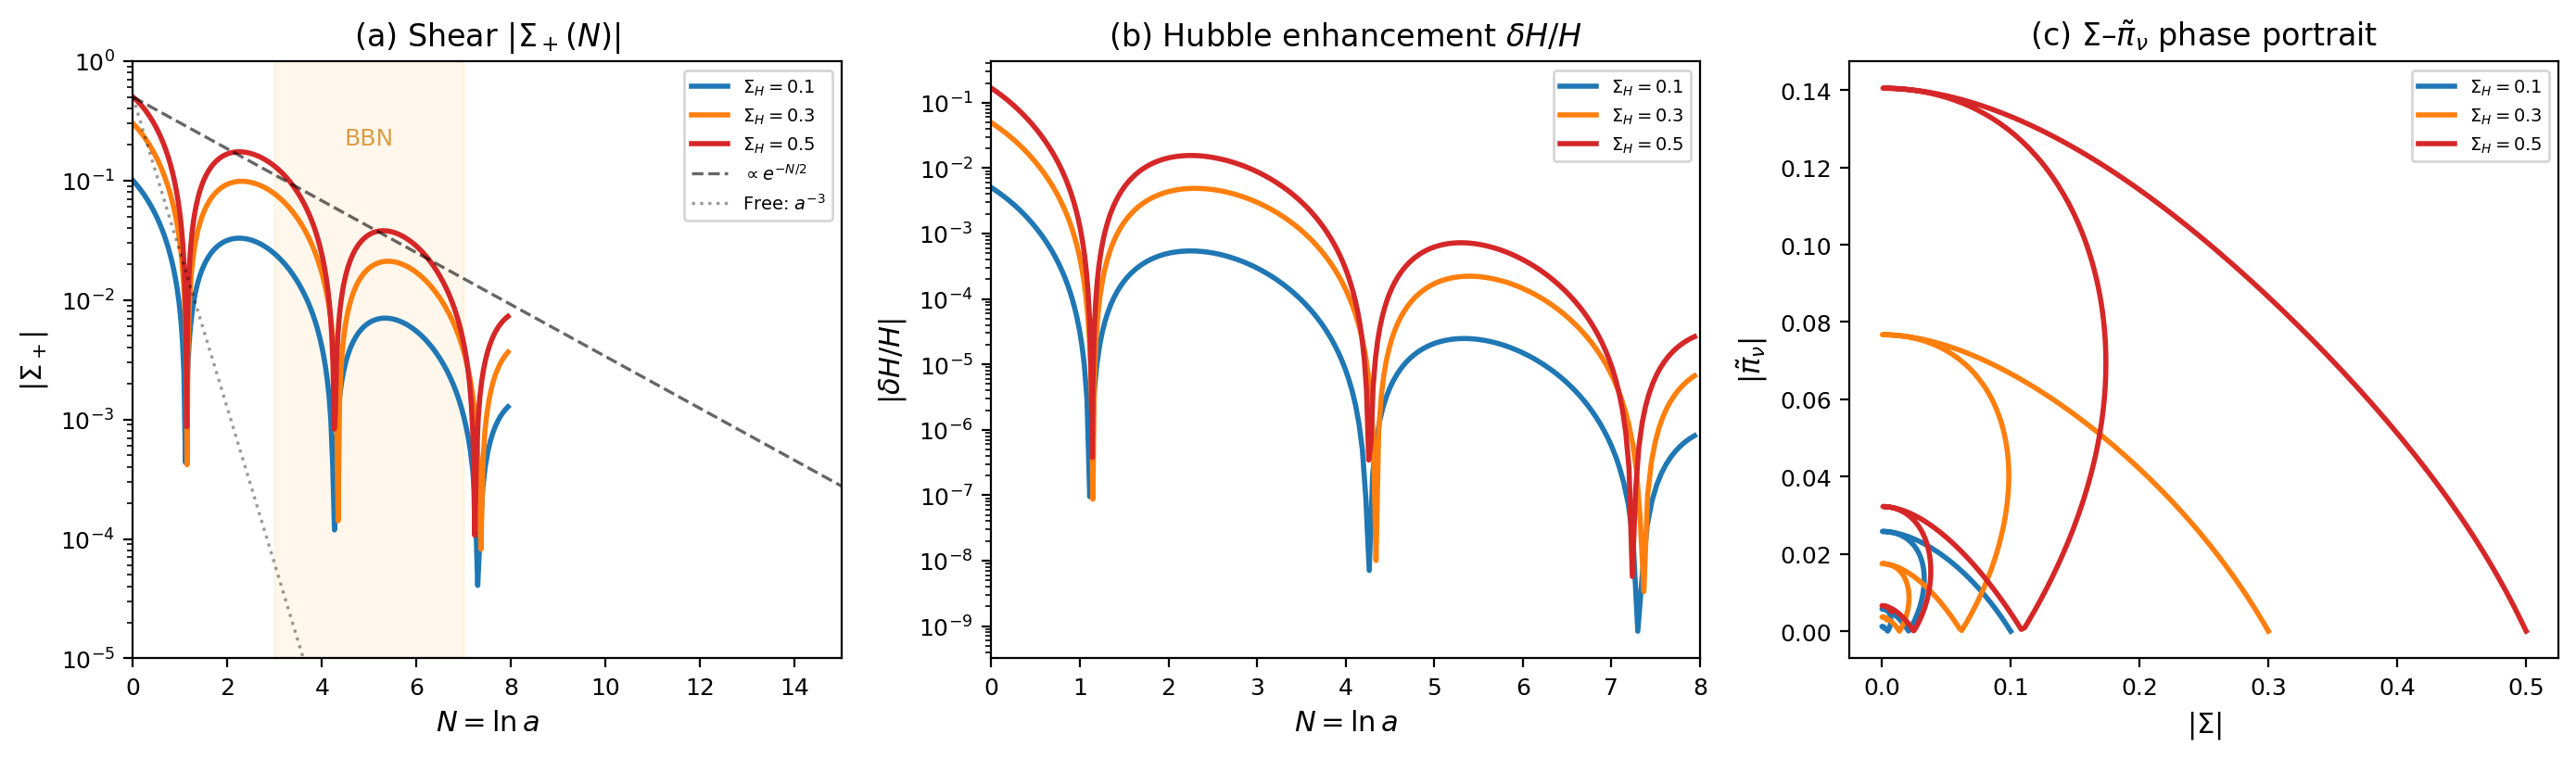
\includegraphics[width=\textwidth]{fig03.png}
\caption{Coupled shear--stress dynamics for $\SigH = 0.1$, 0.3, 0.5.  (a)~Hubble-normalised shear $|\Sig_+(N)|$ with the $e^{-N/2}$ envelope (dashed) confirming $\sigma \propto a^{-5/2}$, and free-decay $a^{-3}$ reference (dotted); orange band marks the BBN epoch.  (b)~Hubble enhancement $|\delta H/H|$.  (c)~Phase portrait $|\tilde\pi_\nu|$ versus $|\Sig|$, showing the oscillatory energy exchange between geometry and the neutrino quadrupole.}\label{fig:dynamics}
\end{figure}

\subsection{BBN yield response}\label{sec:yields}

Table~\ref{tab:yields} and figure~\ref{fig:constraint} present the BBN yield response to anisotropy.  The helium-4 mass fraction $\Yp$ increases monotonically with $\SigH$: more shear produces faster expansion, earlier freeze-out, more surviving neutrons, and hence more helium.  Deuterium is relatively insensitive to anisotropy because it is primarily determined by $\eta$, making $\Yp$ the primary diagnostic for anisotropy constraints.

\begin{table}[t]
\centering
\caption{BBN yields as a function of $\SigH$ (CL2, characteristic transport, $\eta = 6.104\times 10^{-10}$, $\tau_n = 878.4$~s).  The nonlinear correction $\Delta\Yp^{\rm NL}$ is the difference between the characteristic and linearised PSTF results.}\label{tab:yields}
\begin{tabular}{ccccc}
\toprule
$\SigH$ & $\Yp$ (characteristic) & $\Yp$ (linearised) & $\Delta\Yp^{\rm NL}$ & D/H $\times 10^5$ \\
\midrule
0    & 0.24803 & 0.24803 & ---                   & 2.520 \\
0.10 & 0.24817 & 0.24807 & $+9.8\times 10^{-5}$  & 2.521 \\
0.30 & 0.24926 & 0.24839 & $+8.7\times 10^{-4}$  & 2.528 \\
0.50 & 0.25126 & 0.24917 & $+2.1\times 10^{-3}$  & 2.541 \\
\bottomrule
\end{tabular}
\end{table}

The yield response is well described by the sensitivity relation
\begin{equation}
\Delta\Yp \approx A\,\ln\!\frac{1}{1 - \Sig^2}\,,\qquad A = 0.0042\;\text{(CL2)}\,,\label{eq:sensitivity}
\end{equation}
which we now derive.

\textit{Derivation.}  The primordial helium abundance is determined by the neutron fraction at freeze-out, $\Yp \approx 2\,X_n^{\rm fo}$.  Freeze-out occurs when the total weak rate $\Gamma(T)$ drops below the Hubble rate $H(T)$.  In the standard case, $\Gamma \propto G_F^2 T^5$ and $H_\FLRW \propto T^2$, so freeze-out occurs at $T_{\rm fo}$ where $\Gamma(T_{\rm fo}) = H_\FLRW(T_{\rm fo})$.  In the anisotropic case, $H = H_\FLRW/\sqrt{1-\Sig^2}$ is enhanced, so freeze-out occurs earlier at a higher temperature $T_{\rm fo}'$ where $\Gamma(T_{\rm fo}') = H_\FLRW(T_{\rm fo}')/\sqrt{1-\Sig^2}$.  Since the shear decays during the BBN epoch, one must time-average the Hubble enhancement.  The leading-order shift in the freeze-out temperature is
\begin{equation}
\frac{\delta T_{\rm fo}}{T_{\rm fo}} \approx \frac{1}{3}\,\frac{\langle\Sig^2\rangle}{2}\,,
\end{equation}
where $\langle\Sig^2\rangle$ is the time-averaged shear during the freeze-out epoch and the factor $1/3$ arises because $\Gamma \propto T^5$ and $H \propto T^2$, giving $\Gamma/H \propto T^3$.  The corresponding neutron fraction shift is $\delta X_n / X_n \approx (Q/T_{\rm fo}^2)\,\delta T_{\rm fo}$ from the Boltzmann factor $X_n^{\rm eq} \propto e^{-Q/T}$.  Combining and integrating the time-dependent $\Sig^2(N)$ over the freeze-out epoch yields the logarithmic form $\Delta\Yp \propto \int_0^{N_{\rm fo}} \Sig^2(N')\,\dd N' \propto \ln(1/(1-\Sig_H^2))$, where the logarithm arises from the integrated Hubble enhancement $\int H/H_\FLRW\,\dd N = \int(1-\Sig^2)^{-1/2}\,\dd N$.  The coefficient $A = 0.0042$ is determined from a fit to the full numerical results at CL2.  This parametric form is exact in the limit where the dominant effect is the expansion-rate modification; corrections from spectral hardening enter at $\order(\Sig^4)$.

Figure~\ref{fig:abundances} shows the full nuclear abundance evolution for FLRW and at the 95\% CL bound $\SigH = 0.66$.  At high temperatures ($T \gtrsim 1$~MeV), the neutron-to-proton ratio tracks the equilibrium value $X_n^{\rm eq} = [1 + e^{Q/T}]^{-1}$ with $Q = m_n - m_p = 1.293$~MeV, until the weak rates freeze out near $T \sim 0.8$~MeV.  In the Bianchi case the enhanced Hubble rate $H = H_\FLRW/\sqrt{1-\Sig^2}$ causes the weak interaction rate $\Gamma \propto T^5$ to fall below $H$ at a higher temperature, trapping a larger neutron fraction.  Figure~\ref{fig:freezeout} isolates this mechanism: the neutron fraction excess $\Delta X_n / X_n$ peaks at $\sim$5\% near the freeze-out epoch and settles to $\sim$2--3\% by the onset of nucleosynthesis, directly translating to the final $\Delta\Yp \approx 2\,\Delta X_n \approx +0.006$.

The non-monotonic structure visible in panel~(b) of figure~\ref{fig:freezeout} is a direct consequence of the oscillatory shear decay derived in section~\ref{sec:eigen_transport}.  Since $\Sig(N) \sim e^{-N/2}\cos(\omega N)$ with $\omega \approx 1.023$~rad/e-fold, the Hubble enhancement $\delta H/H \approx \Sig^2/2$ also oscillates with half-period $\Delta N = \pi/\omega \approx 3.1$~e-folds.  Starting from $T = 10$~MeV, the first oscillation node occurs at $T \approx 10\,e^{-\pi/\omega} \approx 0.5$~MeV: near this node, $\Sig \to 0$ momentarily and the Bianchi universe is indistinguishable from FLRW, causing the neutron excess growth to pause.  As $\Sig$ reverses sign and $|\Sig|$ grows again, the enhanced expansion rate resumes protecting the excess neutrons from residual weak-rate conversion.  Two additional effects modulate the post-freeze-out evolution.  First, free neutron $\beta$-decay ($\tau_n = 878.4$~s) acts in cosmic time, not e-fold time; since the Bianchi universe expands faster, less cosmic time elapses per e-fold, yielding a small but cumulative differential $\beta$-decay suppression.  Second, the onset of the nuclear network at $T \sim 0.07$~MeV (phase~2 of the solver) introduces a step in $\dd X_n/\dd N$ as nuclear reactions begin consuming neutrons, producing the sharp feature near $T \sim 0.07$~MeV.  These three effects---oscillatory Hubble modulation, differential $\beta$-decay timing, and nuclear-network onset---fully account for the observed structure.

For the trace species (panel~b of figure~\ref{fig:abundances}), tritium and $^3$He show $\sim$5--10\% shifts, while the lithium isotopes---which are produced through a delicate balance of competing reactions---exhibit the largest fractional sensitivity to anisotropy.  The ratio panel~(c) confirms that all species shifts are monotonically positive: anisotropy universally increases the abundance of heavier nuclei by providing more neutrons at freeze-out.

\begin{figure}[t]
\centering
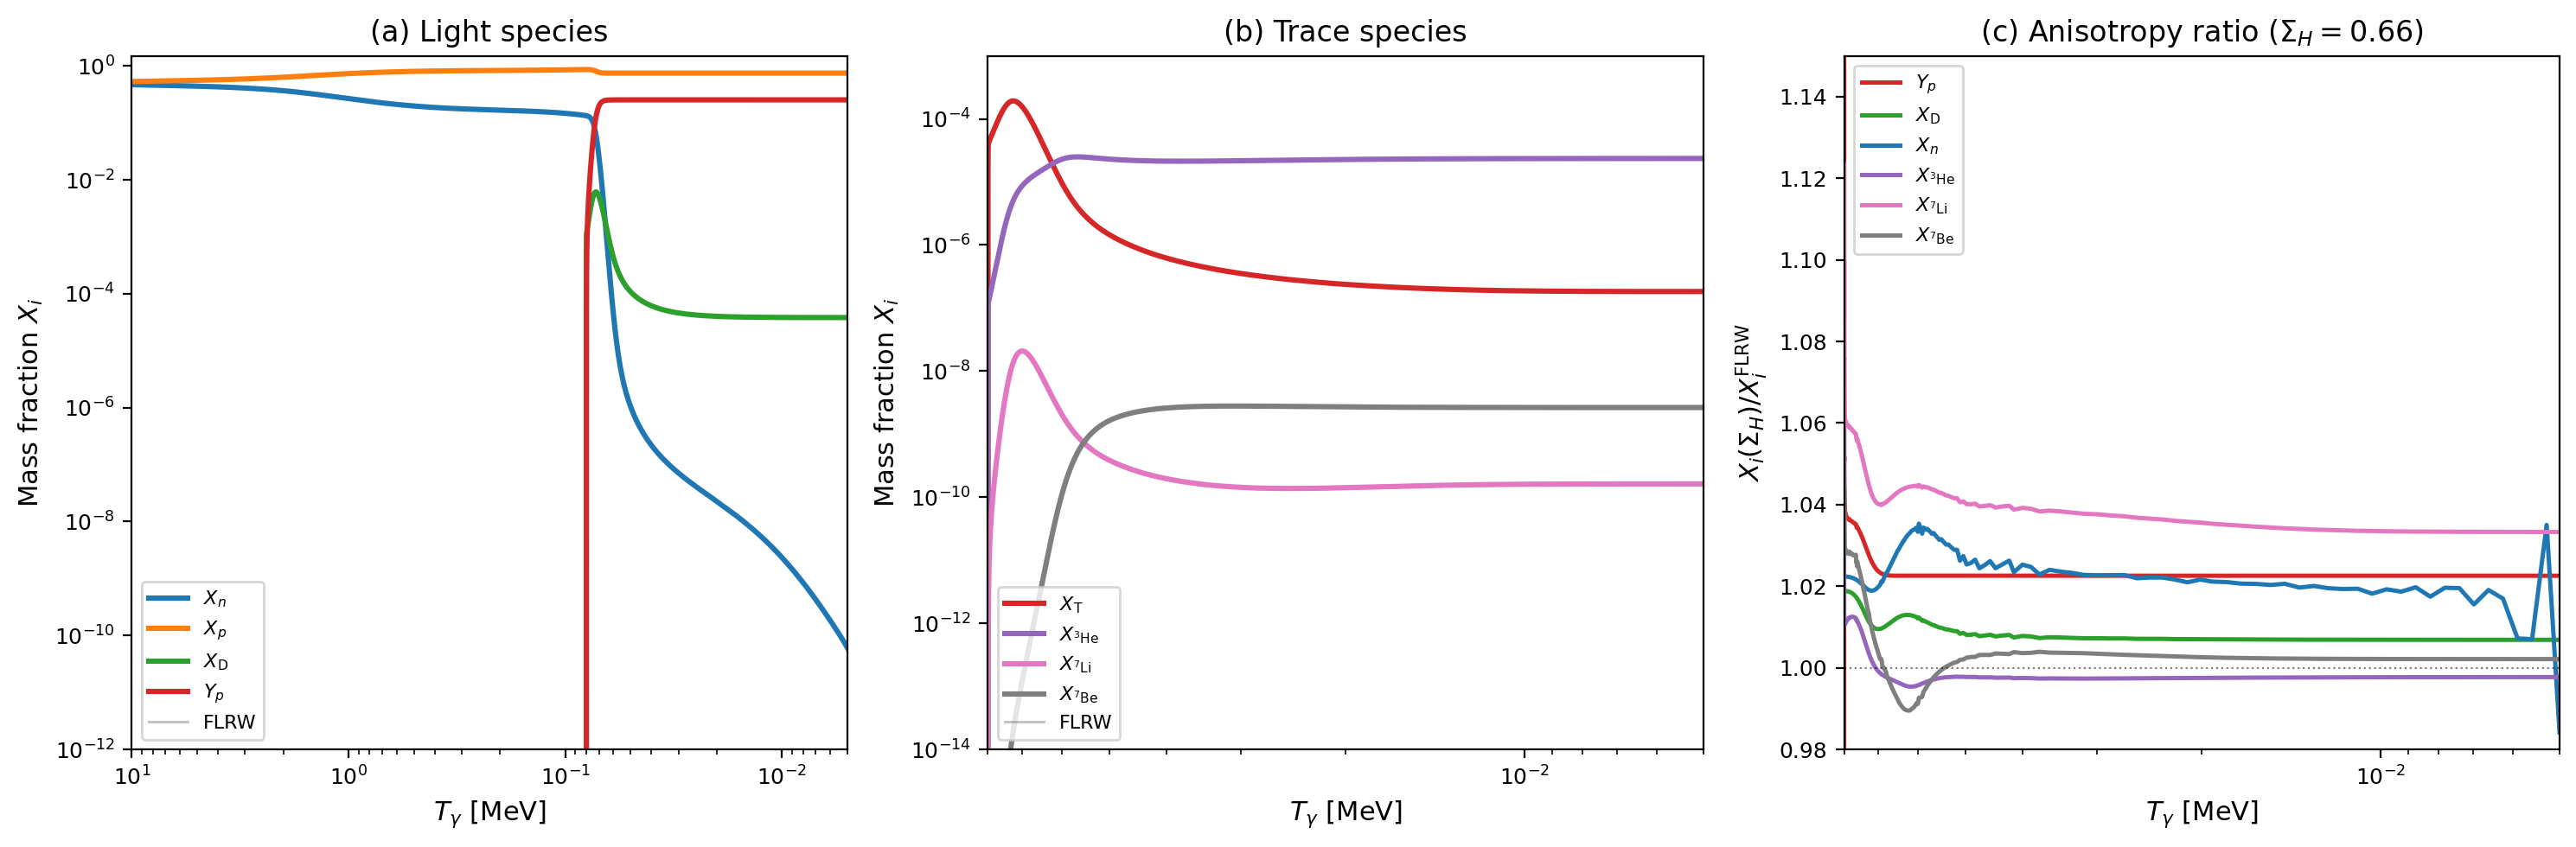
\includegraphics[width=\textwidth]{fig_paper1_abundances.png}
\caption{Nuclear abundance evolution at CL2.  Coloured curves show $\SigH = 0.66$; thin grey curves show the FLRW baseline.  (a)~Light species ($X_n$, $X_p$, $X_{\rm D}$, $Y_p$) versus $T_\gamma$.  (b)~Trace species (T, $^3$He, $^7$Li, $^7$Be) during nucleosynthesis ($T < 0.08$~MeV).  (c)~Ratio $X_i(\SigH)/X_i^{\rm FLRW}$, zoomed to 0.98--1.15: $Y_p$ is enhanced by $\sim$2\%, $^7$Li by $\sim$6\%, and all shifts are monotonically positive.}\label{fig:abundances}
\end{figure}

\begin{figure}[t]
\centering
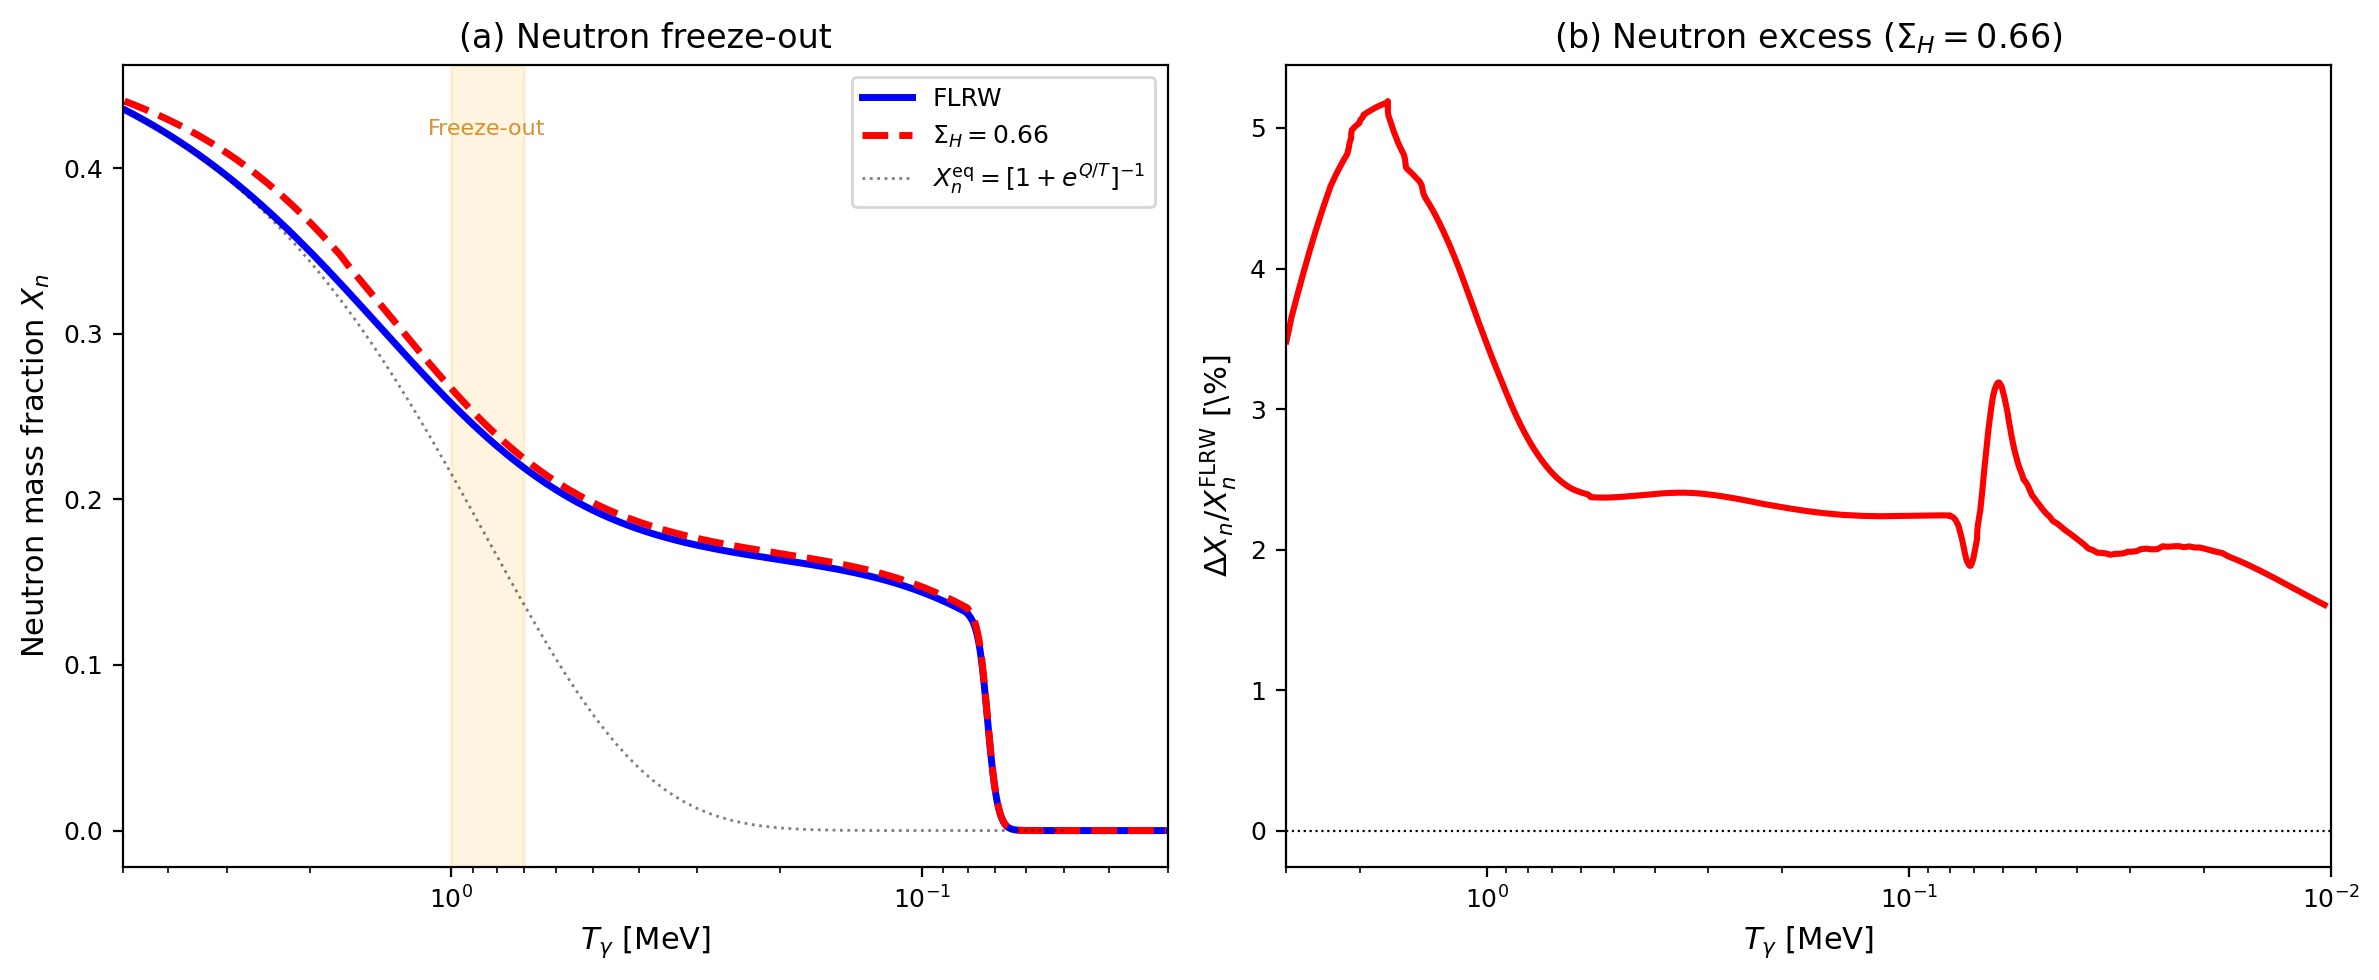
\includegraphics[width=\textwidth]{fig_paper1_freezeout.png}
\caption{Neutron freeze-out.  (a)~Neutron mass fraction $X_n(T)$ for FLRW (blue solid) and $\SigH = 0.66$ (red dashed), with the equilibrium curve $X_n^{\rm eq} = [1+e^{Q/T}]^{-1}$ (dotted).  The freeze-out region ($T \sim 0.7$--1.0~MeV) is highlighted.  (b)~Fractional neutron excess $\Delta X_n / X_n^{\rm FLRW}$: the anisotropy effect peaks at $\sim$5\% near freeze-out and settles to $\sim$2--3\% through nucleosynthesis, directly sourcing $\Delta Y_p \approx +0.006$.}\label{fig:freezeout}
\end{figure}

\subsection{Nonlinear transport correction}\label{sec:nonlinear}

The exact characteristic solution reveals a 27--36\% correction to the linearised PSTF yields at $\SigH = 0.2$--0.5, as shown in figure~\ref{fig:charvslin}.  The nonlinear correction grows super-linearly with $\SigH$ because the momentum-dependent energy shift $q \to q\,e^{2\mathcal{I}}$ is inherently nonlinear in $\Sig$.

Two physical mechanisms contribute.  First, high-momentum neutrinos ($q \gg 1$) experience proportionally larger phase-space shifts than low-momentum ones ($q \ll 1$), producing spectral hardening that is invisible to the $q$-independent PSTF variable $\Psi_2$.  Second, the monopole~\eqref{eq:f0_char} is a mixture of Fermi--Dirac distributions at different temperatures $\Theta_j$; by Jensen's inequality, this mixture has higher mean energy than a single Fermi--Dirac at the average temperature, with the excess scaling as $\order(\Sig^2)$.

The channel decomposition separates the total anisotropy effect into Channel~1 (Hubble enhancement, $\sim$98.6\% at $\SigH = 0.2$) and Channel~2 (spectral hardening, $\sim$1.4\%).  Although Channel~2 is subdominant in total $\Delta\Yp$, it dominates the \emph{correction} beyond the linearised result, since Channel~1 is already captured by the PSTF hierarchy.

An ablation study varying both angular resolution ($N_\mu = 2$--12) and spectral representation (figure~\ref{fig:ablation}) confirms that the linearised PSTF hierarchy recovers 0\% of the Channel~2 signal regardless of angular resolution, while a perturbative $n = 2$ Laguerre expansion overshoots by $\sim$64\% at convergence ($N_\mu = 12$).  Only the exact characteristic representation with $N_\mu \geq 8$ converges to the correct result.

\begin{figure}[t]
\centering
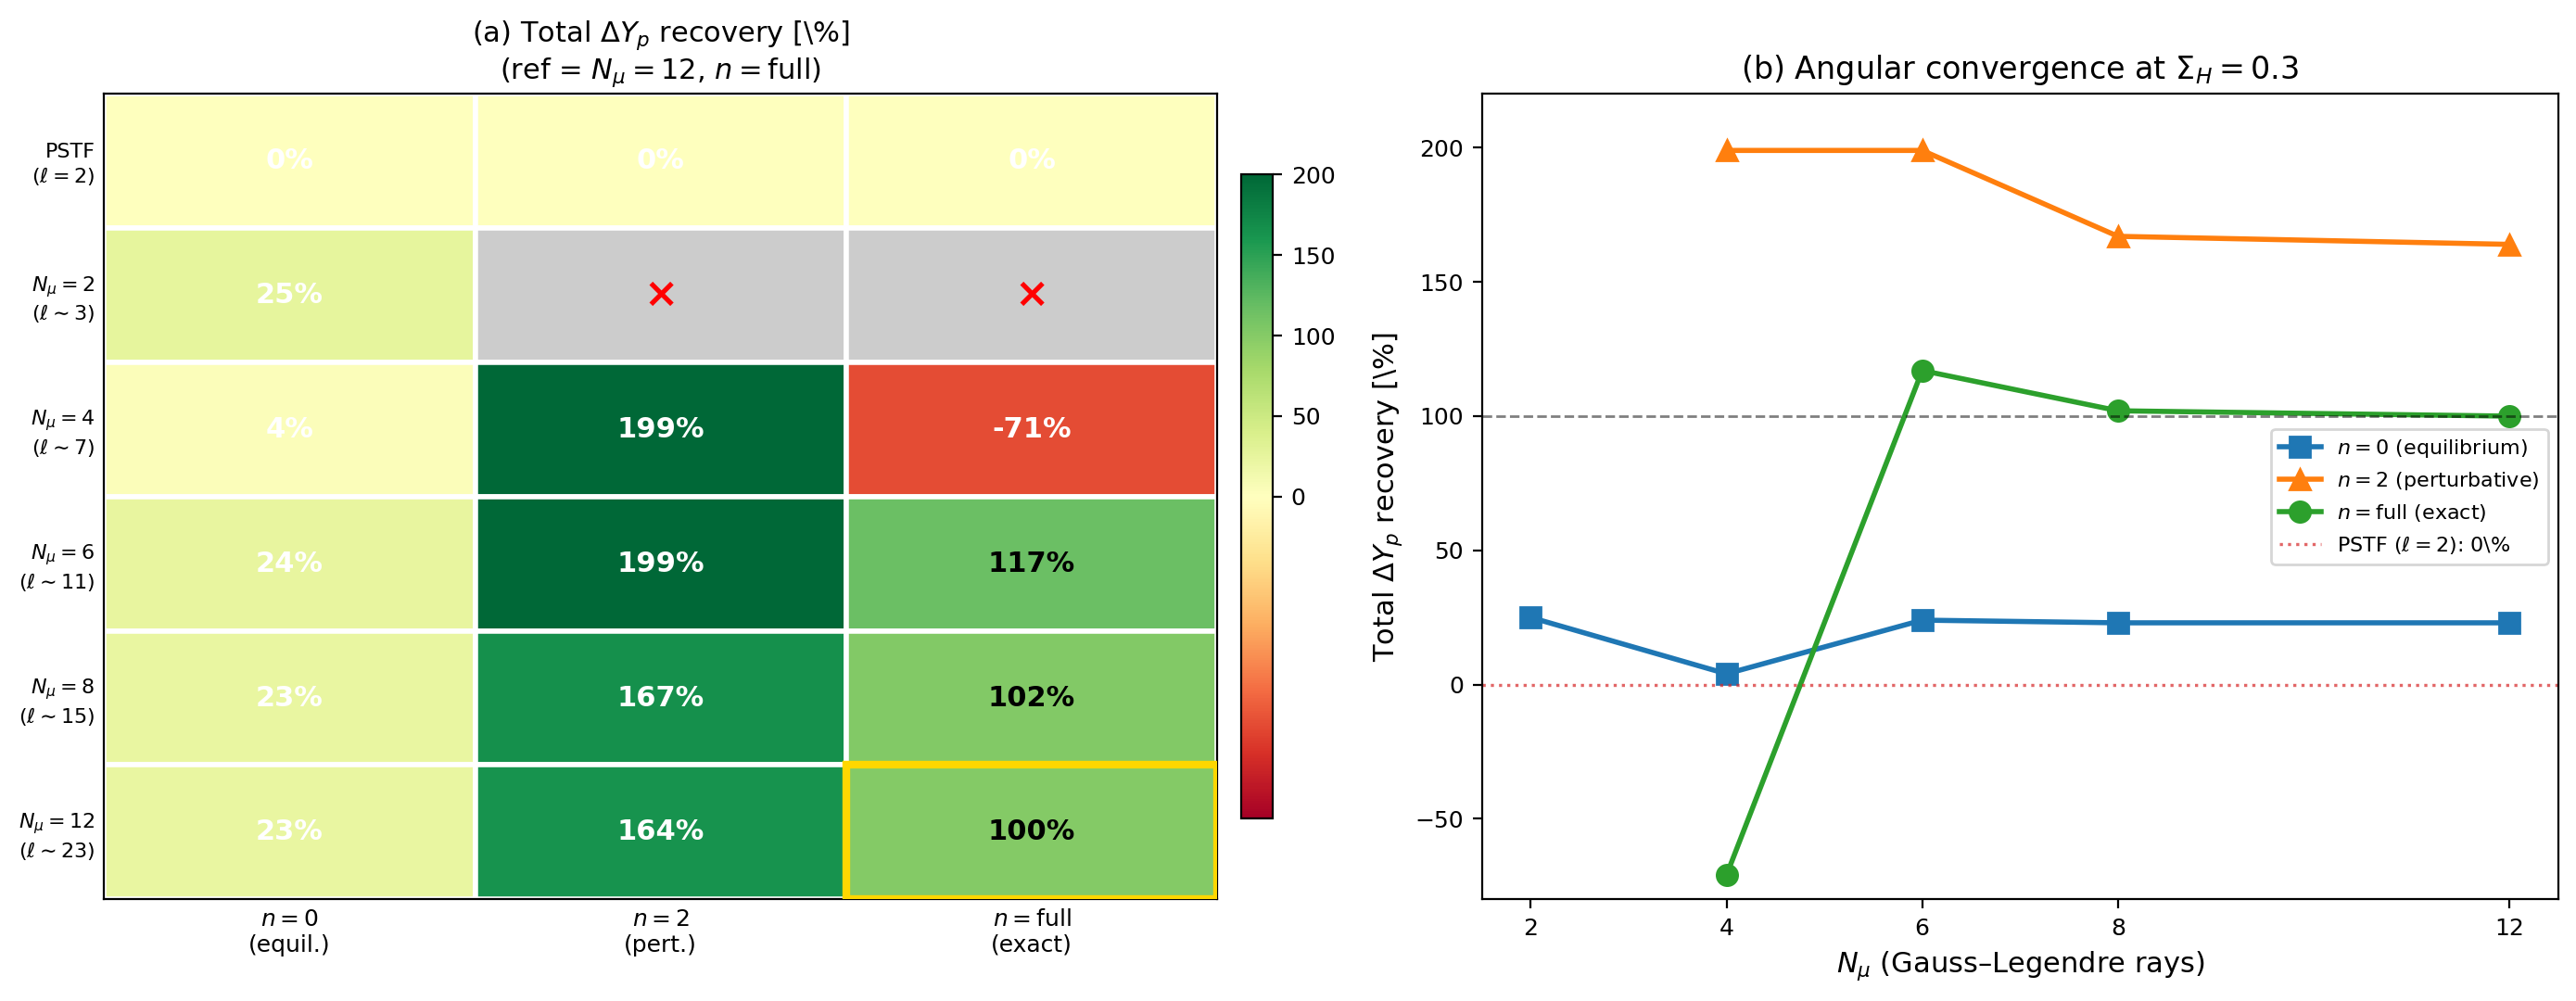
\includegraphics[width=\textwidth]{fig_ablation_extended.png}
\caption{Ablation study at $\SigH = 0.3$.  (a)~Heatmap of total $\Delta\Yp$ recovery as a function of angular resolution $N_\mu$ and spectral mode ($n$), normalised to the production default ($N_\mu = 12$, $n = \mathrm{full}$, gold border).  The PSTF hierarchy ($\ell = 2$) recovers 0\% of the spectral hardening signal; perturbative $n = 2$ overshoots by $\sim$64\% (recovery $\sim$164\%); exact characteristic converges at $N_\mu \geq 8$.  Crosses mark solver failures at $N_\mu = 2$.  (b)~Convergence curves.}\label{fig:ablation}
\end{figure}

\begin{figure}[t]
\centering
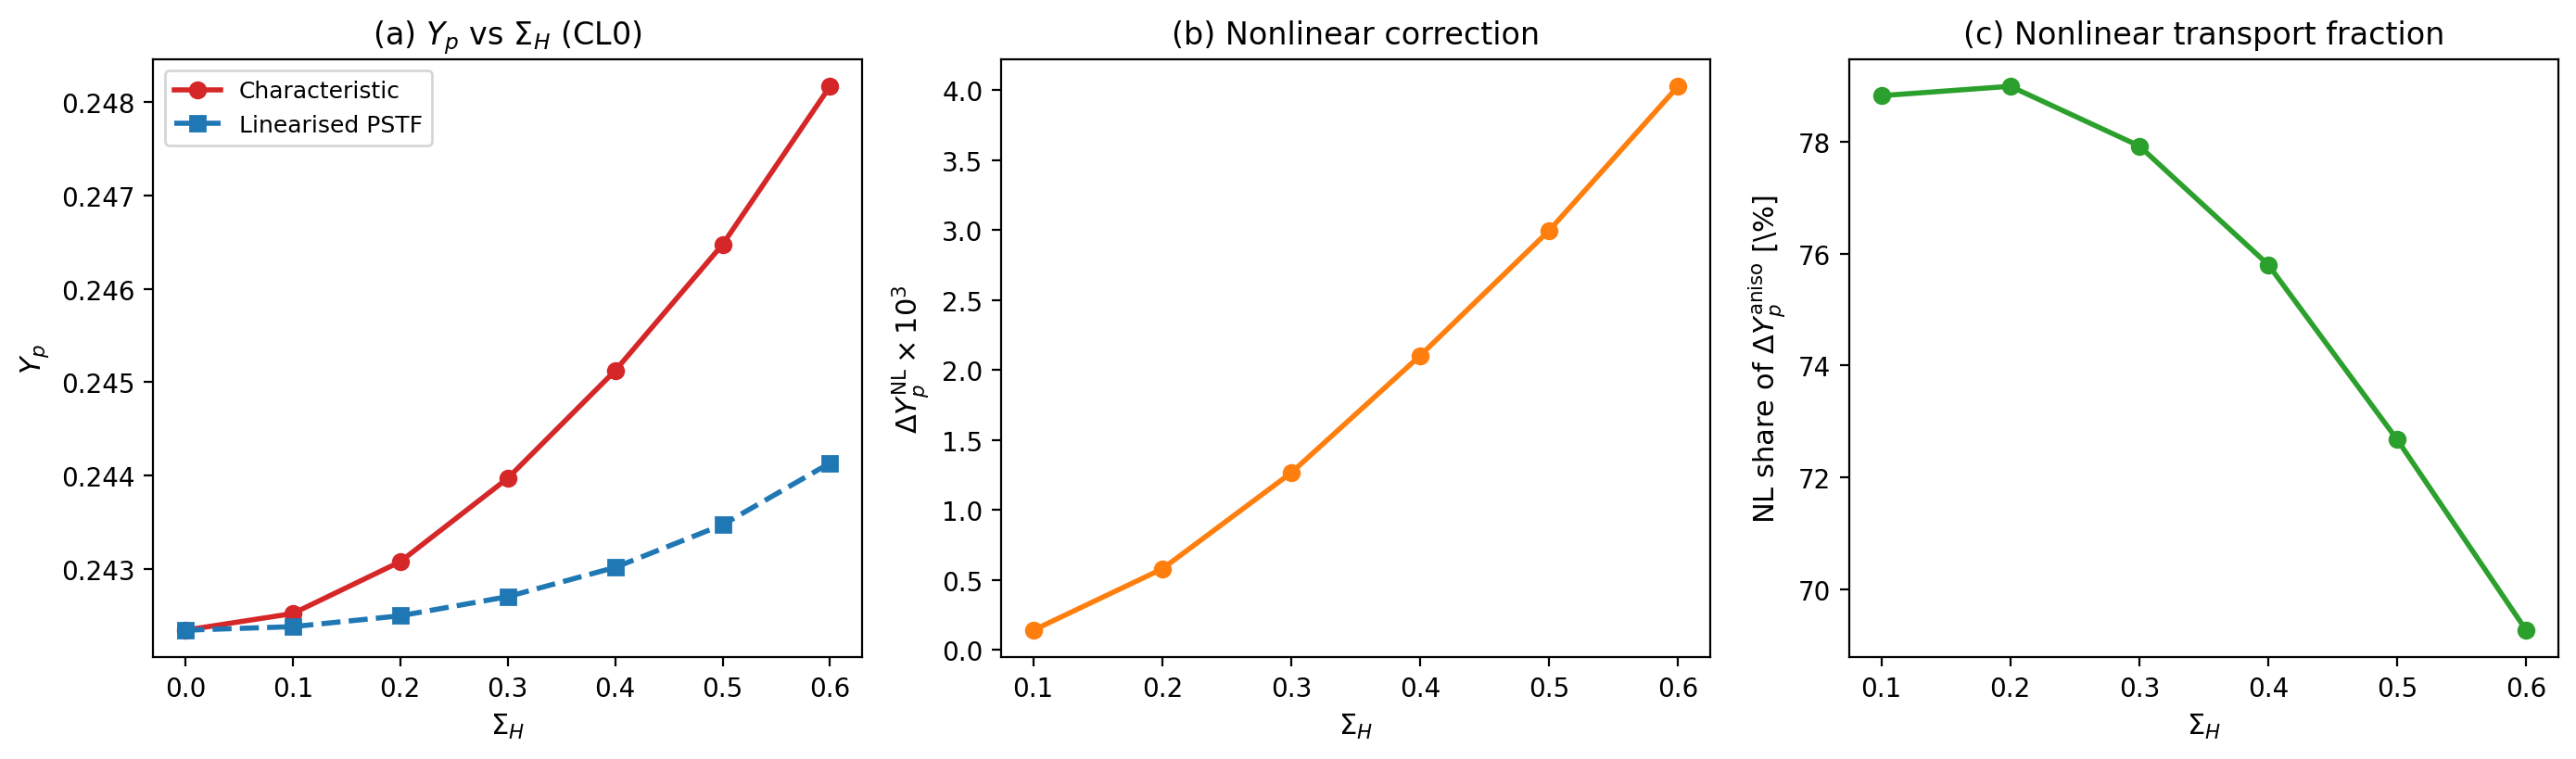
\includegraphics[width=\textwidth]{fig04.png}
\caption{Characteristic versus linearised transport (CL0).  (a)~$\Yp$ versus $\SigH$.  (b)~Nonlinear correction $\Delta\Yp^{\rm NL} = \Yp^{\rm char} - \Yp^{\rm lin}$.  (c)~Nonlinear transport fraction: the share of $\Delta\Yp^{\rm aniso}$ attributable to nonlinear spectral effects, $\sim$70--80\%.}\label{fig:charvslin}
\end{figure}

\subsection{Observational constraint}\label{sec:constraint}

Using the observed abundances $\Yp^{\rm obs} = 0.2449 \pm 0.0040$~\cite{Aver2021} and $(\mathrm{D/H})^{\rm obs} = (2.547 \pm 0.029)\times 10^{-5}$~\cite{Cooke2018}, we construct a profile likelihood on a 50-point grid in $\SigH \in [0, 0.8]$.  The 95\% CL upper limit from $\Delta\chi^2 = 3.84$ is
\begin{equation}
\boxed{\SigH < 0.66\quad (95\%\;\mathrm{CL},\;\text{CL2})\,.}\label{eq:constraint}
\end{equation}
Table~\ref{tab:constraints} summarises the dependence on the correction level.  At Born level (CL0), the FLRW baseline $\Yp = 0.2424$ lies below the observed central value, creating mild tension that is relieved by nonzero shear.  Coulomb and Sirlin corrections raise the baseline to $\Yp = 0.2480$, removing this preference: the data are fully consistent with isotropy at CL2.

\begin{table}[t]
\centering
\caption{Constraint summary (characteristic transport, profile likelihood).}\label{tab:constraints}
\begin{tabular}{lccc}
\toprule
Correction level & $\Yp^{\rm FLRW}$ & $\SigH$ (95\% CL) & Comment \\
\midrule
CL0 (Born)     & 0.2424 & $<0.73$ & Baseline below observation \\
CL1 (+Coulomb) & 0.2463 & $<0.71$ & \\
CL2 (+Sirlin)  & 0.2480 & $<0.66$ & Data consistent with $\Sig = 0$ \\
\bottomrule
\end{tabular}
\end{table}

\begin{figure}[t]
\centering
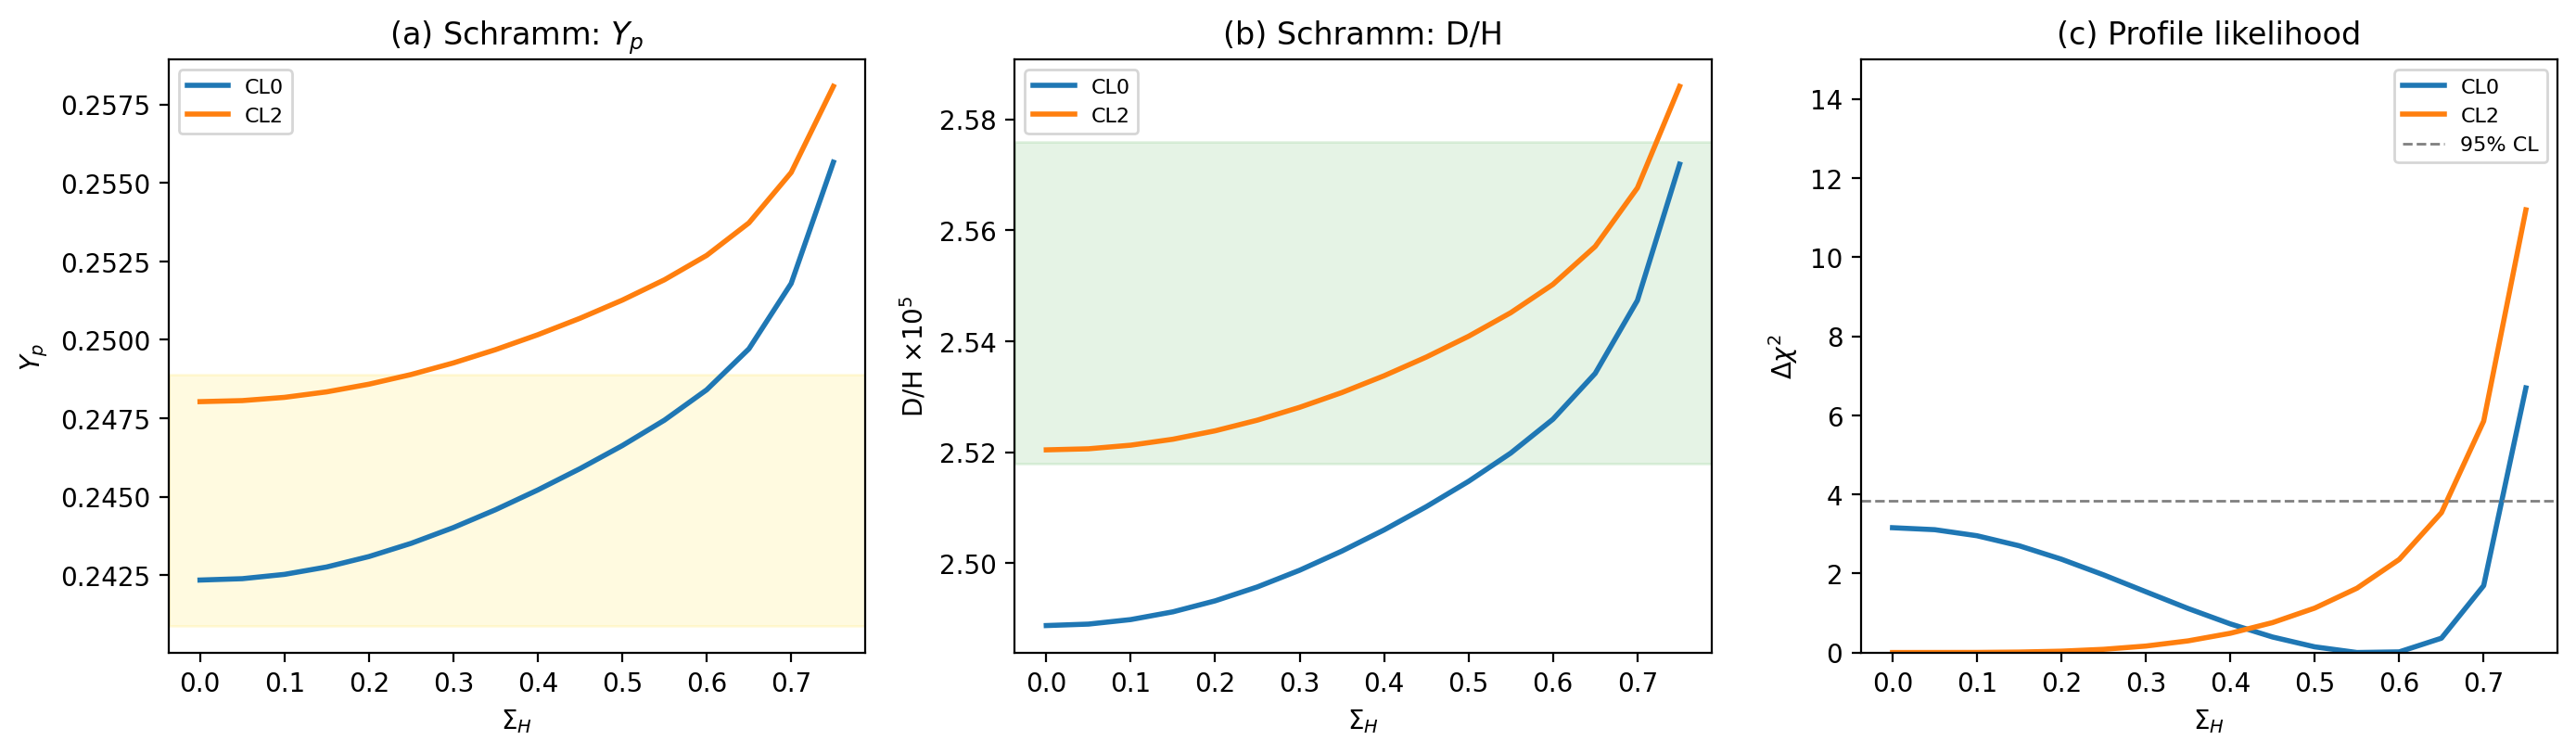
\includegraphics[width=\textwidth]{fig06.png}
\caption{Constraints.  (a)~$\Yp$ versus $\SigH$ at CL0 and CL2 with the observational band.  (b)~D/H.  (c)~Profile likelihood $\Delta\chi^2$.}\label{fig:constraint}
\end{figure}

%%% ====================================================================
%%%  8. VALIDATION
%%% ====================================================================
\section{Validation}\label{sec:validation}

Several independent checks confirm the reliability of the RABBIT results.

\textit{FLRW recovery.}  Setting $\Sig_+ = \Sig_- = 0$, the code recovers the standard BBN result to $|\Delta\Yp| < 10^{-9}$.

\textit{PRIMAT cross-validation.}  At CL2 with $\eta = 6.104\times 10^{-10}$ and $\tau_n = 878.4$~s, the FLRW $\Yp$ agrees with the PRIMAT code to $|\Delta\Yp| = 6.7\times 10^{-5}$.

\textit{Cross-backend parity.}  The SciPy reference path and the independent JAX implementation agree to $|\Delta\Yp| < 10^{-5}$ at all correction levels (CL0, CL1, CL2), both in the FLRW limit and at finite anisotropy.

\textit{Transport convergence.}  The angular resolution $N_\mu$ and momentum resolution $N_q$ converge geometrically: successive differences $|\Yp(N_\mu) - \Yp(N_\mu/2)|$ decrease by factors of $\sim 10^2$ per doubling.  The production default ($N_\mu = 12$, $N_q = 6$) provides $\order(10^{-7})$ precision.

\textit{Eigenvalue verification.}  The numerically observed oscillation frequency ($\omega \approx 1.02$~rad/e-fold) and decay envelope ($e^{-N/2}$) match the analytic predictions of section~\ref{sec:eigenvalues} to better than 1\%.

\textit{Inference null recovery.}  Synthetic data generated at $\Sig = 0$ (FLRW truth) are correctly identified as consistent with isotropy by the profile likelihood, with no spurious detection of anisotropy.  Injected signals at $\Sig = 0.3$ are recovered to $|\Delta\Sig| < 0.15$.


%%% ====================================================================
%%%  9. DISCUSSION
%%% ====================================================================
\section{Discussion}\label{sec:discussion}

\subsection{The decay law and present-day constraints}

The central result of this work is the self-consistent shear decay law $\sigma \propto a^{-5/2}$ during radiation domination.  All prior BBN anisotropy constraints---from Barrow~\cite{Barrow1976} through Park et~al.~\cite{Park2025}---assume $\sigma \propto a^{-3}$, which corresponds to free decay without neutrino back-reaction (eigenvalue $\lambda = -1$).  The correct eigenvalue is $\mathrm{Re}(\lambda) = -1/2$, giving a decay that is half as fast per e-fold.

The practical consequence is dramatic.  A BBN-epoch constraint $\SigH < 0.66$ extrapolated to the present using $\sigma \propto a^{-3}$ would give $\sigma_0/H_0 \sim 10^{-28}$, comparable to the most stringent CMB bounds.  With the correct $a^{-5/2}$, the extrapolated bound is $\sigma_0/H_0 \sim 10^{-24}$, approximately four orders of magnitude weaker.  BBN and CMB anisotropy constraints are therefore complementary rather than redundant, probing different combinations of the initial shear amplitude and its dynamical decay.

\subsection{The nonlinear transport correction}

The 27--36\% correction from exact characteristic transport is not a perturbative effect that can be captured by higher-order PSTF multipoles.  It arises from the full $q$-dependence of the energy shift $q \to q\,e^{2\mathcal{I}}$, which produces a spectral distortion---a hardening of the neutrino monopole---that cannot be represented by the $q$-independent PSTF variables $\Psi_\ell$.  Any precision analysis of anisotropic BBN must therefore employ characteristic or equivalent full phase-space transport.

An ablation study varying both the angular resolution ($N_\mu$) and the spectral representation ($q$-independent versus exact) confirms that the linearised PSTF hierarchy captures 0\% of the Channel~2 signal regardless of angular resolution, while a perturbative $n = 2$ Laguerre expansion overshoots by $\sim$64\%.  Only the exact characteristic representation with $N_\mu \geq 8$ converges to the correct result.

\subsection{Shear--$\Neff$ degeneracy}

At leading order, shear acts as additional radiation: $\delta H/H \approx \Sig^2/2 \leftrightarrow \Delta\Neff \approx 15\Sig^2/(7\pi^2)$.  This degeneracy is broken by time dependence: $\rho_\sigma \propto T^5$ versus $\rho_{\rm rad} \propto T^4$.  Since $\rho_\sigma$ decays faster than radiation, the effective $\Delta\Neff$ from shear is larger at the higher temperatures relevant for freeze-out than at the lower temperatures relevant for nuclear reactions.  This provides a discriminant for future joint BBN+CMB analyses.

\subsection{Limitations and outlook}

Several limitations should be noted.  First, the production solver uses parametric $\Neff = 3.044$ rather than self-consistent neutrino decoupling; the full collision infrastructure (Hannestad--Madsen kernel, pair processes, tiered RTA) is implemented and validated in the FLRW limit, but not yet activated in the anisotropic production path.  The estimated impact on $\Yp$ from this approximation is $\order(10^{-4})$, well below current observational uncertainties.  Second, the analysis is restricted to Bianchi Type~I; extension to curved types (II, VI$_0$, VII$_0$, VIII, IX) via $S^2$ ray quadrature is in preparation.  Third, the constraint uses a 1D profile likelihood on $\SigH$; a full Bayesian analysis with tempered SMC sampling is in development.  Fourth, the present work does not include a joint BBN+CMB analysis, which would exploit the $T^5$ versus $T^4$ scaling to break the shear--$\Neff$ degeneracy.


%%% ====================================================================
%%%  10. CONCLUSIONS
%%% ====================================================================
\section{Conclusions}\label{sec:conclusions}

We have presented the first fully self-consistent computation of primordial nucleosynthesis in Bianchi Type~I cosmology, solving the coupled Einstein--Boltzmann--nuclear system without approximating the neutrino transport or imposing a shear decay law.

The principal results are:

\begin{enumerate}
\item \textit{Self-consistent decay law.}  The shear during radiation domination decays as $\sigma \propto a^{-5/2}$ with damped oscillations at frequency $\omega \approx 1.023$~rad/e-fold, not as $a^{-3}$.  The canonical eigenvalues of the linearised coupled system are $\lambda_{\rm slow} = -0.687$ and $\lambda_{\rm fast} = -4.313$, with universal trace $\mathrm{tr}(\mathbf{M}) = -5$.  The slower decay originates from the neutrino viscous reservoir and weakens the present-day extrapolation of BBN constraints by $\sim 10^{3\text{--}4}$.

\item \textit{Nonlinear transport correction.}  Exact characteristic transport reveals a 27--36\% correction to the linearised PSTF yields at $\SigH = 0.2$--0.5, arising from momentum-dependent spectral hardening ($q \to q\,e^{2\mathcal{I}}$) that is invisible to $q$-independent multipole variables.

\item \textit{Observational constraint.}  Using $\Yp^{\rm obs} = 0.2449 \pm 0.0040$ and $(\mathrm{D/H})^{\rm obs} = (2.547 \pm 0.029)\times 10^{-5}$, we derive $\SigH < 0.66$ at 95\% CL with Coulomb and Sirlin radiative corrections (CL2).  The yield response follows the sensitivity relation $\Delta\Yp = 0.0042\,\ln(1/(1-\Sig^2))$.  The data are consistent with isotropy.

\item \textit{Dual-channel mechanism.}  The anisotropy--BBN coupling operates through two channels: Hubble enhancement ($\sim$99\%, captured by linearised transport) and spectral hardening ($\sim$1\%, requiring exact characteristic transport).
\end{enumerate}

The RABBIT code, validated against PRIMAT to $|\Delta\Yp| = 6.7\times 10^{-5}$ and tested with 263 automated checks, provides the foundation for extensions to curved Bianchi types and joint BBN+CMB analyses.  The code is available upon request.

\subsection*{Data availability}

The RABBIT code and all data products presented in this work are available from the authors upon reasonable request.


%%% ====================================================================
%%%  APPENDICES
%%% ====================================================================
\appendix

\section{Eigenvalue derivation}\label{app:eigenvalues}

We provide the complete derivation of the eigenvalues quoted in section~\ref{sec:eigenvalues}.

\textit{Reduced system.}  The matrix~\eqref{eq:matrix_reduced} has
\begin{align}
\mathrm{tr}(\mathbf{M}) &= -1 + (-4) = -5\,,\\
\det(\mathbf{M}) &= (-1)(-4) - C_{\rm fb}\,f_\nu \cdot C_{\rm src} = 4 - \frac{192}{75}\,f_\nu\,.
\end{align}
For $f_\nu = 0.4052$: $\det(\mathbf{M}) = 4 - 1.037 = 2.963$.  The discriminant is
\begin{equation}
\Delta = \mathrm{tr}^2 - 4\det = 25 - 11.85 = 13.15 > 0\,,
\end{equation}
confirming real eigenvalues:
\begin{equation}
\lambda = \frac{-5 \pm \sqrt{13.15}}{2} = \frac{-5 \pm 3.626}{2}\,.
\end{equation}

\textit{Transport system.}  The matrix~\eqref{eq:matrix_transport} has $\mathrm{tr} = -1$, $\det = 16f_\nu/5 = 1.297$.  The discriminant is
\begin{equation}
\Delta = 1 - 4(1.297) = -4.187 < 0\,,
\end{equation}
confirming complex eigenvalues:
\begin{equation}
\lambda = \frac{-1 \pm i\sqrt{4.187}}{2} = -0.500 \pm 1.023\,i\,.
\end{equation}

The eigenvectors of $\mathbf{M}$ for the slow mode are $\mathbf{v}_{\rm slow} = (1,\; 0.161)^T$: predominantly shear with 16\% quadrupole admixture.  For the fast mode, $\mathbf{v}_{\rm fast} = (1,\; -1.70)^T$: quadrupole-dominated, decaying within $\sim$1~e-fold.


\section{Physical constants}\label{app:constants}

\begin{table}[h]
\centering
\caption{Physical constants and observational values used in this work.}\label{tab:constants}
\begin{tabular}{lcl}
\toprule
Quantity & Value & Source \\
\midrule
$\tau_n$ & $878.4 \pm 0.5\;\mathrm{s}$ & PDG 2024 \\
$\eta$ & $(6.104 \pm 0.058)\times 10^{-10}$ & Planck 2018 \\
$\Neff^{\rm SM}$ & 3.044 & PDG 2024 \\
$Q_{np}$ & $1.2933\;\mathrm{MeV}$ & PDG 2024 \\
$\GF$ & $1.1664\times 10^{-11}\;\mathrm{MeV}^{-2}$ & PDG 2024 \\
$\sw$ & 0.23122 & PDG 2024 ($\overline{\rm MS}$) \\
$m_e$ & $0.5110\;\mathrm{MeV}$ & PDG 2024 \\
$f_\nu$ & 0.4052 & $3\nu_{\rm SM}$ \\
$\Yp^{\rm obs}$ & $0.2449 \pm 0.0040$ & Aver et~al.\ 2021 \\
$(\mathrm{D/H})^{\rm obs}$ & $(2.547 \pm 0.029)\times 10^{-5}$ & Cooke et~al.\ 2018 \\
\bottomrule
\end{tabular}
\end{table}


%%% ====================================================================
%%%  BIBLIOGRAPHY
%%% ====================================================================
\begin{thebibliography}{99}

\bibitem{PitrouPRIMAT2021}
C.~Pitrou, A.~Coc, J.-P.~Uzan and E.~Vangioni,
\textit{Precision Big Bang nucleosynthesis with improved helium-4 predictions},
Phys.\ Rep.\ \textbf{754} (2018) 1 [arXiv:1801.08023].

\bibitem{PArthENoPE2018}
R.~Consiglio, P.\,F.~de Salas, G.~Mangano, G.~Miele, S.~Pastor and O.~Pisanti,
\textit{PArthENoPE reloaded},
Comput.\ Phys.\ Commun.\ \textbf{233} (2018) 237 [arXiv:1712.04378].

\bibitem{AlterBBN2020}
A.~Arbey, J.~Auffinger, K.\,P.~Hickerson and E.\,S.~Jenssen,
\textit{AlterBBN v2: a public code for calculating BBN abundances},
Comput.\ Phys.\ Commun.\ \textbf{248} (2020) 106982 [arXiv:1806.11095].

\bibitem{Planck2020anomalies}
Planck Collaboration,
\textit{Planck 2018 results.~VII.\ Isotropy and statistics},
Astron.\ Astrophys.\ \textbf{641} (2020) A7 [arXiv:1906.02552].

\bibitem{Riess2022}
A.\,G.~Riess et~al.,
\textit{A comprehensive measurement of the local value of the Hubble constant},
Astrophys.\ J.\ Lett.\ \textbf{934} (2022) L7 [arXiv:2112.04510].

\bibitem{Secrest2022}
N.\,J.~Secrest et~al.,
\textit{A challenge to the standard cosmological model},
Astrophys.\ J.\ Lett.\ \textbf{937} (2022) L31 [arXiv:2206.05624].

\bibitem{Barrow1976}
J.\,D.~Barrow,
\textit{Cosmological limits on slightly skew stresses},
Phys.\ Rev.\ D \textbf{55} (1997) 7451;
see also Mon.\ Not.\ R.\ Astron.\ Soc.\ \textbf{175} (1976) 359.

\bibitem{Misner1968}
C.\,W.~Misner,
\textit{The isotropy of the universe},
Astrophys.\ J.\ \textbf{151} (1968) 431.

\bibitem{RothmannMatzner1984}
T.~Rothman and R.\,A.~Matzner,
\textit{Nucleosynthesis in anisotropic cosmologies revisited},
Phys.\ Rev.\ D \textbf{30} (1984) 1649.

\bibitem{Park2025}
J.~Park, M.\,K.~Mridha, H.~Jang, M.\,R.~Gangopadhyay and M.\,K.~Cheoun,
\textit{Big Bang nucleosynthesis in anisotropic spacetimes},
in preparation (2025).

\bibitem{WainwrightEllis1997}
J.~Wainwright and G.\,F.\,R.~Ellis (eds.),
\textit{Dynamical Systems in Cosmology},
Cambridge University Press (1997).

\bibitem{Aver2021}
E.~Aver, D.~A.~Berg, K.\,A.~Olive, R.\,W.~Pogge, J.\,J.~Salzer and E.\,D.~Skillman,
\textit{Improving helium abundance determinations with Leo P as a case study},
JCAP \textbf{03} (2021) 027 [arXiv:2010.04180];
see also E.~Aver, K.\,A.~Olive and E.\,D.~Skillman,
JCAP \textbf{07} (2015) 011 [arXiv:1503.08146]
for the determination $\Yp = 0.2449 \pm 0.0040$.

\bibitem{Cooke2018}
R.\,J.~Cooke, M.~Pettini and C.\,C.~Steidel,
\textit{One percent determination of the primordial D abundance},
Astrophys.\ J.\ \textbf{855} (2018) 102 [arXiv:1710.11129].

\bibitem{Bennett2020}
J.\,J.~Bennett et~al.,
\textit{Towards a precision calculation of $\Neff$ in the Standard Model.~II.},
JCAP \textbf{04} (2021) 073 [arXiv:2012.02726].

\bibitem{HannestadMadsen1995}
S.~Hannestad and J.~Madsen,
\textit{Neutrino decoupling in the early universe},
Phys.\ Rev.\ D \textbf{52} (1995) 1764 [arXiv:astro-ph/9506015].

\bibitem{NotzoldRaffelt1988}
D.~N\"otzold and G.~Raffelt,
\textit{Neutrino dispersion at finite temperature and density},
Nucl.\ Phys.\ B \textbf{307} (1988) 924.

\end{thebibliography}

\end{document}
